\section{Breve historia de la óptica cuántica}

    A finales del siglo XIX la física clásica se erguía como un edificio de una solidez que hoy resulta difícil de imaginar. La mecánica de Newton daba cuenta del movimiento de los planetas con una precisión que había permitido descubrir Neptuno con la punta del lápiz antes que con el telescopio, la termodinámica había domesticado el calor y las máquinas, y las cuatro ecuaciones que Maxwell publicó en 1865 habían unificado la electricidad, el magnetismo y la luz en una sola teoría capaz de predecir la existencia de ondas que Hertz produjo en su laboratorio veinte años más tarde. Tan completo parecía el edificio que Lord Kelvin, en una conferencia pronunciada en 1900, pudo decir que en el cielo despejado de la física solo quedaban dos pequeñas nubes. Una de ellas era el resultado negativo del experimento de Michelson y Morley y desembocaría en la relatividad; la otra era el problema de la distribución espectral de la radiación del cuerpo negro, y de ella salió la mecánica cuántica.

    Este capítulo se ocupa de esa segunda nube y de todo lo que salió de ella, pero hay que advertir desde el principio que la historia no transcurrió como suele contarse. La versión resumida afirma que Planck cuantizó la luz en 1900, que Einstein lo confirmó en 1905 con el efecto fotoeléctrico y que desde entonces el fotón es parte del mobiliario de la física. Cada uno de esos tres enunciados es falso o, en el mejor de los casos, engañoso. Planck no cuantizó la luz sino los osciladores materiales de las paredes de la cavidad, y siguió creyendo durante más de una década que el campo electromagnético era estrictamente continuo; Einstein sí cuantizó la luz en 1905, pero su argumento principal no fue el efecto fotoeléctrico sino un razonamiento termodinámico sobre la entropía de la radiación; y la comunidad tardó casi veinte años en aceptar la existencia de los cuantos de luz, hasta que el experimento de Compton en 1923 hizo insostenible la resistencia. Reconstruiremos con detalle cada uno de esos episodios en la sección siguiente, porque el orden lógico de los argumentos es mucho más instructivo que el resumen.

    La historia posterior es más conocida. El modelo atómico que Niels Bohr propuso en 1913 postulaba órbitas electrónicas estables y transiciones entre ellas con emisión o absorción de un cuanto de energía $h\nu$, vinculando por primera vez la estructura de la materia con la naturaleza discreta de la radiación y explicando de paso la fórmula empírica que Balmer había hallado para el hidrógeno en 1885. La década de 1920 trajo la mecánica cuántica propiamente dicha, con la hipótesis de de Broglie sobre las ondas de materia, la mecánica matricial de Heisenberg, la mecánica ondulatoria de Schrödinger y la síntesis de ambas que hemos desarrollado en el capítulo anterior. Ninguna de esas construcciones, sin embargo, cuantizaba el campo electromagnético: en todas ellas la luz seguía siendo un campo clásico externo que actuaba sobre átomos cuánticos, aproximación que hoy llamamos semiclásica y que sigue siendo suficiente para una parte considerable de la óptica.

    El paso decisivo lo dio Paul Dirac en 1927, en un artículo cuyo título anuncia exactamente su contenido, \textit{La teoría cuántica de la emisión y absorción de radiación} \citep{dirac1927quantum}. Dirac tomó el campo electromagnético libre, lo descompuso en modos normales, observó que cada modo es formalmente un oscilador armónico y aplicó a cada uno de ellos el procedimiento de cuantización canónica, que es precisamente el programa que desarrollaremos en este capítulo. El resultado fue que las excitaciones del campo aparecen en unidades discretas, de manera que el fotón dejó de ser una hipótesis sobre la naturaleza de la luz y pasó a ser una consecuencia aritmética del formalismo. Dirac obtuvo además, en el mismo trabajo, la tasa de emisión espontánea que Einstein había tenido que introducir a mano en 1917, y con ello resolvió el problema que había dejado abierto durante una década: la emisión espontánea no es espontánea en absoluto, sino emisión estimulada por las fluctuaciones del vacío.

    La teoría así construida, la electrodinámica cuántica, tropezó de inmediato con un obstáculo formidable. Al calcular cantidades observables como la autoenergía del electrón, es decir, la energía de su interacción con su propio campo, o la polarización del vacío debida a la creación de pares virtuales, los resultados divergían. La solución llegó tras la Segunda Guerra Mundial con la técnica de renormalización desarrollada de forma independiente por Richard Feynman, Julian Schwinger y Sin-Itiro Tomonaga, quienes compartieron el premio Nobel de 1965. La idea central es que los parámetros que figuran en las ecuaciones, la masa y la carga \textit{desnudas}, no son los que se miden en el laboratorio, pues las interacciones con las fluctuaciones del vacío \textit{visten} a la partícula; absorbiendo los infinitos en una redefinición de esos parámetros, las cantidades observables resultan finitas. Hans Bethe había mostrado el camino en 1947 con un cálculo no relativista del desplazamiento de Lamb realizado, según cuenta la anécdota, en el tren de vuelta de la conferencia de Shelter Island.

    Los triunfos experimentales de la electrodinámica cuántica renormalizada la convirtieron en la teoría física más precisa jamás construida, y citamos los dos que fijaron su reputación.

    \begin{enumerate}
        \item El desplazamiento de Lamb. En 1947 Willis Lamb y Robert Retherford midieron una pequeña diferencia de energía entre los niveles $2S_{1/2}$ y $2P_{1/2}$ del hidrógeno, que según la ecuación de Dirac debían ser exactamente degenerados. La electrodinámica cuántica, al incluir la interacción del electrón con las fluctuaciones del vacío, predijo ese corrimiento con gran exactitud, y con ello demostró que el vacío cuántico tiene consecuencias medibles.

        \item El momento magnético anómalo del electrón. La teoría de Dirac predice un factor $g$ exactamente igual a dos, y en 1947 Polykarp Kusch y Henry Foley midieron una desviación de una parte por mil. Schwinger calculó en 1948 la primera corrección radiativa, obteniendo $g/2 = 1 + \alpha/2\pi$, en acuerdo con la medida. Hoy el cálculo se ha llevado hasta el quinto orden en $\alpha$ y el acuerdo entre teoría y experimento alcanza las doce cifras significativas, lo que equivale a medir la distancia entre Bogotá y Bucaramanga con un error del tamaño de un átomo.
    \end{enumerate}

    Los diagramas que Feynman introdujo para organizar estos cálculos proporcionaron además una herramienta visual que convirtió manipulaciones perturbativas de enorme complejidad en un procedimiento casi mecánico, y su influencia sobre la manera de pensar de los físicos ha sido tan grande como la de los propios resultados.

    Con la electrodinámica cuántica firmemente establecida, la óptica cuántica pudo nacer como disciplina propia, y su acta de nacimiento tiene una fecha precisa: 1960, cuando Theodore Maiman hizo funcionar el primer láser de rubí. Antes de esa fecha, todas las fuentes de luz disponibles eran térmicas, es decir, caóticas, y la naturaleza cuántica del campo quedaba enmascarada por el desorden estadístico; el láser proporcionó por primera vez luz intensa, monocromática y coherente, y con ella la posibilidad de preparar y medir estados del campo con un control que antes era impensable.

    La teoría correspondiente llegó de inmediato. En 1963 Roy Glauber publicó la formulación cuántica de la coherencia óptica que hemos anticipado al final del capítulo anterior \citep{glauber1963quantum}, introduciendo las funciones de correlación de orden arbitrario y los \textit{estados coherentes} que estudiaremos en este capítulo, que son los estados del campo cuantizado que más se parecen a una onda clásica y que describen la luz de un láser ideal; ese mismo año George Sudarshan demostró que todo estado del campo admite una representación diagonal en la base de estados coherentes \citep{sudarshan1963equivalence}. Glauber recibió el premio Nobel en 2005 por este trabajo.

    El paso siguiente fue encontrar luz que ninguna teoría clásica pudiera explicar. En 1977 Jeff Kimble, Mario Dagenais y Leonard Mandel observaron el \textit{antiagrupamiento} de fotones en la fluorescencia de resonancia de un solo átomo, es decir, que los fotones llegan al detector de uno en uno y nunca en parejas, comportamiento estrictamente imposible para cualquier campo clásico por argumentos que discutiremos al tratar el experimento de Grangier, Roger y Aspect. En 1985 Richard Slusher y colaboradores generaron los primeros estados comprimidos, en los cuales el ruido cuántico de una de las cuadraturas del campo se reduce por debajo del nivel del vacío a costa de aumentarlo en la otra, respetando así la relación de indeterminación pero burlando el límite que parecía imponer. Esos estados dejaron de ser una curiosidad de laboratorio el día en que los detectores de ondas gravitacionales empezaron a usarlos: desde 2019 LIGO inyecta luz comprimida en sus interferómetros y con ello aumenta en un factor apreciable el volumen de universo que puede observar.

    La relación entre la electrodinámica cuántica y la óptica cuántica es la que existe entre una teoría fundamental y un campo de exploración. La primera proporciona el marco conceptual y las reglas de cálculo para la interacción entre radiación y materia cargada; la segunda estudia los fenómenos que emergen de esa interacción cuando la naturaleza cuántica de la luz es dominante, y ha servido a la vez como el banco de pruebas más exigente de las predicciones de la teoría y como el motor que ha llevado a la información cuántica, a la metrología de precisión y a la manipulación de sistemas cuánticos individuales. El resto de este capítulo construye el formalismo que hace posible todo eso, empezando por el principio, es decir, por la pregunta de por qué fue necesario abandonar la descripción clásica de la luz.

\section{La luz nunca ha sido clásica}

    La sección anterior ha adelantado que el orden lógico de los argumentos que condujeron a la cuantización de la luz difiere bastante del relato habitual. Vamos a reconstruir ahora ese orden con todo el detalle de los cálculos, porque cada uno de los tres episodios, el de Planck, el de Einstein y el de Compton, añade un ingrediente distinto y porque la naturaleza exacta de lo que cada uno demostró es lo que suele perderse en los resúmenes.

    \subsection{El problema del cuerpo negro}

        Un \textit{cuerpo negro} es, por definición, un objeto que absorbe toda la radiación que incide sobre él, sin reflejar ni transmitir nada. Gustav Kirchhoff demostró en 1860 un teorema de gran alcance sobre estos objetos: en equilibrio térmico, la razón entre el poder emisivo y el poder absorbente de cualquier cuerpo es una función universal de la frecuencia y de la temperatura, independiente del material del que esté hecho. Para un cuerpo negro, cuyo poder absorbente es la unidad, el poder emisivo \textit{es} esa función universal, de manera que determinar el espectro de un cuerpo negro equivale a determinar una función de la naturaleza y no una propiedad de una sustancia particular. Esa universalidad es lo que convirtió el problema en el más importante de la física teórica de finales del siglo XIX.

        La realización experimental de un cuerpo negro es una cavidad cerrada con un pequeño orificio: la radiación que entra por el orificio rebota tantas veces en el interior que su probabilidad de volver a salir es despreciable, de modo que el orificio absorbe todo y se comporta como una superficie perfectamente negra. Lo que se mide es la radiación que escapa por él, y esa radiación es una muestra del campo electromagnético en equilibrio térmico con las paredes. El problema del cuerpo negro es, por tanto, el problema de determinar la densidad espectral de energía del campo electromagnético encerrado en una cavidad a temperatura $T$, y así lo abordaremos, con las herramientas de la teoría electromagnética y sin recurrir a la mecánica estadística más que en el único punto donde resulta imprescindible.

            Consideremos una cavidad cúbica de lado $L$ con paredes perfectamente conductoras. Las condiciones de frontera que impone la electrodinámica son que la componente tangencial del campo eléctrico se anule sobre cada pared, pues un conductor perfecto no soporta campo tangencial en su superficie. Dentro de la cavidad el campo satisface la ecuación de onda que dedujimos del sistema de Maxwell,
            \begin{equation}\label{eq:OndaCavidadBB}
                \nabla^{2}\mathbf{E} - \frac{1}{c^{2}}\frac{\partial^{2}\mathbf{E}}{\partial t^{2}} = 0 ,
            \end{equation}
            y buscamos soluciones estacionarias, es decir, ondas estacionarias de frecuencia bien definida. Separando variables y escogiendo el origen en un vértice de la cavidad, la componente $x$ del campo que se anula sobre las cuatro paredes perpendiculares a $\hat{y}$ y $\hat{z}$ tiene la forma
            \begin{equation}\label{eq:ModoEstacionario}
                E_{x} = E_{0x}\cos\left(k_{x}x\right)\sin\left(k_{y}y\right)\sin\left(k_{z}z\right)\sin\left(\omega t\right),
            \end{equation}
            y análogamente para las otras dos componentes permutando cíclicamente los índices. La función seno se anula en el origen automáticamente, y para que se anule también en la pared opuesta, situada en $y = L$, hace falta que $k_{y}L$ sea un múltiplo entero de $\pi$. Repitiendo el argumento en las tres direcciones,
            \begin{equation}\label{eq:CuantizacionK}
                k_{x} = \frac{n_{x}\pi}{L}, \qquad k_{y} = \frac{n_{y}\pi}{L}, \qquad k_{z} = \frac{n_{z}\pi}{L},
                \qquad n_{x},n_{y},n_{z} \in \{0,1,2,\ldots\},
            \end{equation}
            con la restricción de que a lo sumo uno de los tres enteros puede anularse, pues si dos de ellos se anulan el campo \eqref{eq:ModoEstacionario} es idénticamente nulo. Sustituyendo \eqref{eq:ModoEstacionario} en \eqref{eq:OndaCavidadBB} se obtiene la relación de dispersión
            \begin{equation}\label{eq:DispersionBB}
                \frac{\omega^{2}}{c^{2}} = k_{x}^{2}+k_{y}^{2}+k_{z}^{2} = \frac{\pi^{2}}{L^{2}}\left(n_{x}^{2}+n_{y}^{2}+n_{z}^{2}\right),
                \qquad\text{es decir}\qquad
                \nu = \frac{c}{2L}\sqrt{n_{x}^{2}+n_{y}^{2}+n_{z}^{2}} .
            \end{equation}

            Hasta aquí todo es electrodinámica pura: no hemos usado nada más que las ecuaciones de Maxwell y la condición de conductor perfecto. Lo que necesitamos ahora es contar cuántos modos caben en un intervalo de frecuencias dado, y para ello observemos que cada modo queda etiquetado por un punto de coordenadas enteras no negativas $(n_{x},n_{y},n_{z})$ en un espacio auxiliar. Según \eqref{eq:DispersionBB}, todos los modos con frecuencia menor o igual que $\nu$ son los puntos contenidos en la porción de esfera de radio
            \begin{equation}\label{eq:RadioN}
                n = \sqrt{n_{x}^{2}+n_{y}^{2}+n_{z}^{2}} = \frac{2L\nu}{c}
            \end{equation}
            que cae en el octante de coordenadas positivas, pues los tres enteros son no negativos. Como los puntos de coordenadas enteras tienen densidad unidad en ese espacio, su número es igual al volumen del octante, tal como ilustra la figura \ref{fig:ConteoModos},
            \begin{equation}\label{eq:VolumenOctante}
                \mathcal{N}_{\text{espacial}}(\nu) = \frac{1}{8}\cdot\frac{4}{3}\pi n^{3} = \frac{\pi}{6}\left(\frac{2L\nu}{c}\right)^{3} = \frac{4\pi L^{3}\nu^{3}}{3c^{3}} .
            \end{equation}
            Falta un factor de dos: a cada vector de onda le corresponden dos estados de polarización independientes, porque el campo es transversal y el plano perpendicular a $\mathbf{k}$ es bidimensional. Este es otro ingrediente estrictamente electromagnético y no estadístico. Por tanto
            \begin{equation}\label{eq:ConteoTotal}
                \mathcal{N}(\nu) = 2\,\mathcal{N}_{\text{espacial}}(\nu) = \frac{8\pi L^{3}\nu^{3}}{3c^{3}} .
            \end{equation}
            Derivando respecto de la frecuencia y dividiendo por el volumen $V = L^{3}$ obtenemos la \textit{densidad de modos por unidad de volumen y de frecuencia},
            \begin{equation}\label{eq:DensidadModos}
                \boxed{\;g(\nu) = \frac{1}{V}\frac{d\mathcal{N}}{d\nu} = \frac{8\pi\nu^{2}}{c^{3}} .\;}
            \end{equation}

            \begin{figure}[htbp]
                \centering
                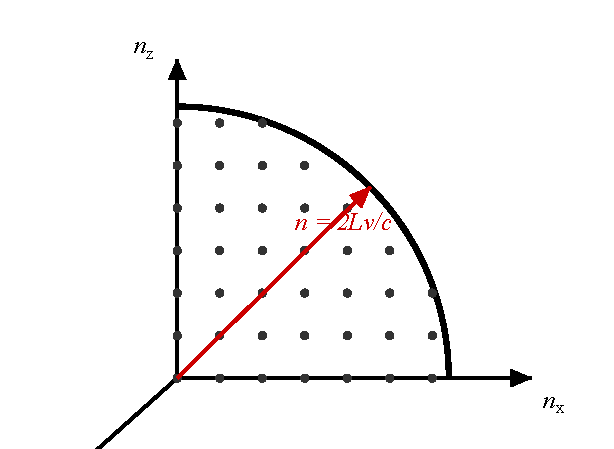
\includegraphics[width=0.5\linewidth]{Capitulo 5/Figuras/ConteoModos.pdf}
                \caption{Conteo de los modos de la cavidad. Cada terna de enteros no negativos $(n_{x},n_{y},n_{z})$ etiqueta un modo, y los que tienen frecuencia menor que $\nu$ llenan el octante de radio $n = 2L\nu/c$, de manera que su número es el volumen de ese octante.}
                \label{fig:ConteoModos}
            \end{figure}

            En \eqref{eq:DensidadModos} está ya contenida toda la dificultad. El número de maneras distintas en que el campo puede oscilar dentro de la cavidad crece como el cuadrado de la frecuencia y no tiene cota superior: por muy alta que sea la frecuencia considerada, siempre caben más modos por encima de ella, y de hecho cada vez más. Este crecimiento sin límite es una consecuencia inevitable de que el campo electromagnético sea un medio continuo con infinitos grados de libertad, uno por cada punto del espacio, tal como discutimos en el capítulo de mecánica analítica al pasar de la cadena discreta al continuo. La densidad de modos es independiente de la forma de la cavidad y del material de las paredes, como exige el teorema de Kirchhoff, y puede demostrarse que el resultado \eqref{eq:DensidadModos} vale para cualquier recinto suficientemente grande comparado con la longitud de onda.

            Para obtener la densidad espectral de energía $\rho(\nu,T)$, es decir, la energía por unidad de volumen y de frecuencia, basta multiplicar el número de modos por la energía media que cada modo posee en equilibrio térmico,
            \begin{equation}\label{eq:EstructuraRho}
                \rho(\nu,T) = g(\nu)\,\overline{\varepsilon}(\nu,T) = \frac{8\pi\nu^{2}}{c^{3}}\,\overline{\varepsilon}(\nu,T).
            \end{equation}
            Este es el único punto en el que la electrodinámica no basta y hay que apelar a la física térmica, y vale la pena subrayarlo: toda la disputa entre la física clásica y la cuántica se reduce a qué se ponga en el lugar de $\overline{\varepsilon}$.

            La respuesta clásica es el teorema de equipartición, según el cual en equilibrio térmico cada grado de libertad cuadrático de un sistema posee una energía media $k_{B}T/2$. Un modo del campo es un oscilador armónico, y como tal tiene dos grados de libertad cuadráticos, la amplitud y su derivada temporal, o equivalentemente los términos eléctrico y magnético de la energía, de manera que
            \begin{equation}\label{eq:Equiparticion}
                \overline{\varepsilon}_{\text{clásica}} = 2\cdot\frac{1}{2}k_{B}T = k_{B}T,
            \end{equation}
            independientemente de la frecuencia del modo. Sustituyendo \eqref{eq:Equiparticion} en \eqref{eq:EstructuraRho} obtenemos la \textit{ley de Rayleigh y Jeans},
            \begin{equation}\label{eq:RayleighJeans}
                \boxed{\;\rho_{\text{RJ}}(\nu,T) = \frac{8\pi\nu^{2}}{c^{3}}\,k_{B}T .\;}
            \end{equation}

            Esta expresión, deducida por Lord Rayleigh en 1900 y corregida en su factor numérico por James Jeans en 1905, es correcta en el límite de frecuencias bajas y concuerda allí con los datos experimentales; pero es catastrófica en todo lo demás. Para verlo, calculemos la energía total contenida en la cavidad por unidad de volumen, que se obtiene integrando sobre todas las frecuencias,
            \begin{equation}\label{eq:CatastrofeIntegral}
                u_{\text{RJ}}(T) = \int_{0}^{\infty}\rho_{\text{RJ}}(\nu,T)\,d\nu = \frac{8\pi k_{B}T}{c^{3}}\int_{0}^{\infty}\nu^{2}\,d\nu = \frac{8\pi k_{B}T}{c^{3}}\left[\frac{\nu^{3}}{3}\right]_{0}^{\infty} = \infty .
            \end{equation}
            La integral diverge, y diverge además de la peor manera posible, pues lo hace en el extremo de frecuencias altas y como un cubo. Paul Ehrenfest bautizó este desastre en 1911 con el nombre que ha quedado: la \textit{catástrofe ultravioleta}.

            Lo que dice \eqref{eq:CatastrofeIntegral} no es un desacuerdo cuantitativo con el experimento sino un absurdo físico. La predicción clásica afirma que cualquier cavidad a cualquier temperatura por encima del cero absoluto contiene una cantidad infinita de energía, y que un cuerpo a temperatura ambiente debería emitir con intensidad creciente en el ultravioleta, en los rayos X y en los rayos gamma. Abrir un horno equivaldría a recibir una descarga letal de radiación. El origen del absurdo es transparente a la luz del cálculo que hemos hecho: hay infinitos modos de frecuencia arbitrariamente alta, según \eqref{eq:DensidadModos}, y la equipartición asigna a cada uno la misma energía $k_{B}T$, de manera que la energía total es infinita por la sencilla razón de que se está repartiendo una porción fija entre un número infinito de receptores. No hay ningún error en el cálculo: el conteo de modos es electrodinámica correcta y la equipartición es mecánica estadística correcta, de modo que la contradicción demuestra que alguna de las dos teorías es falsa fuera de su dominio.

            Por el otro extremo del espectro, Wilhelm Wien había propuesto en 1896 una fórmula empírica que ajustaba muy bien los datos de frecuencia alta,
            \begin{equation}\label{eq:LeyWien}
                \rho_{\text{W}}(\nu,T) = \alpha\,\nu^{3}\,e^{-\beta\nu/T},
            \end{equation}
            con $\alpha$ y $\beta$ constantes por determinar, pero que fallaba por completo en el infrarrojo, donde predice una densidad que tiende a cero mientras que las medidas de Rubens y Kurlbaum en el laboratorio de Berlín mostraban un crecimiento lineal con la temperatura. La situación en octubre de 1900 era, pues, la siguiente: dos fórmulas, cada una correcta en la mitad del espectro y catastróficamente falsa en la otra mitad, y ninguna deducible de principios generales aceptables.

            Max Planck llevaba seis años trabajando en el problema desde una perspectiva termodinámica, estudiando no el campo sino los \textit{resonadores} materiales de las paredes, es decir, los osciladores cargados que absorben y emiten radiación y que mantienen el equilibrio térmico con ella. El 19 de octubre de 1900 presentó ante la Sociedad Física Alemana una fórmula de interpolación entre los dos regímenes conocidos, y en la noche del 7 de diciembre, tras semanas de lo que él mismo describió como el trabajo más intenso de su vida, encontró la manera de deducirla. El precio fue una hipótesis que le resultaba profundamente desagradable y que calificó, en una carta escrita años después, como \textit{un acto de desesperación}.

            \begin{Assumption}[Hipótesis cuántica de Planck]\label{sup:Planck}
                Un resonador material de frecuencia $\nu$ no puede poseer una energía arbitraria, sino únicamente un múltiplo entero de una cantidad elemental proporcional a su frecuencia,
                \begin{equation}\label{eq:HipotesisPlanck}
                    \varepsilon_{n} = n\,h\nu, \qquad n = 0,1,2,\ldots,
                \end{equation}
                donde $h$ es una constante universal.
            \end{Assumption}

            Es indispensable subrayar el alcance exacto de este supuesto, porque es el punto que el relato habitual distorsiona. \textbf{La cuantización \eqref{eq:HipotesisPlanck} se aplica a los osciladores mecánicos de las paredes de la cavidad y no al campo electromagnético}, que para Planck seguía siendo la onda continua de Maxwell, capaz de transportar cualquier cantidad de energía. Lo que está cuantizado es el intercambio: la materia solo puede ceder o recibir energía en paquetes de tamaño $h\nu$, del mismo modo que una máquina expendedora solo acepta monedas de cierto valor aunque el dinero en abstracto sea divisible. Planck fue explícito y reiterado en este punto durante años, y de hecho combatió la hipótesis del cuanto de luz de Einstein hasta bien entrada la década de 1910; en la carta de recomendación que en 1913 escribió para la admisión de Einstein en la Academia Prusiana, tras elogiar sin reservas su obra, pidió que no se le tuviese demasiado en cuenta el haber \textit{errado el blanco} con su hipótesis de los cuantos de luz.

            Podemos ahora calcular la energía media de un resonador bajo el supuesto \ref{sup:Planck}. Este es el único lugar del desarrollo en que necesitamos física estadística, y basta con el ingrediente más elemental de ella, el factor de Boltzmann, según el cual la probabilidad de que un sistema en equilibrio a temperatura $T$ se encuentre en un estado de energía $\varepsilon$ es proporcional a $e^{-\varepsilon/k_{B}T}$. La energía media es entonces el promedio pesado
            \begin{equation}\label{eq:MediaPlanck1}
                \overline{\varepsilon} = \frac{\displaystyle\sum_{n=0}^{\infty}\varepsilon_{n}\,e^{-\varepsilon_{n}/k_{B}T}}{\displaystyle\sum_{n=0}^{\infty}e^{-\varepsilon_{n}/k_{B}T}}
                = \frac{\displaystyle\sum_{n=0}^{\infty}n h\nu\,e^{-nh\nu/k_{B}T}}{\displaystyle\sum_{n=0}^{\infty}e^{-nh\nu/k_{B}T}} ,
            \end{equation}
            donde la diferencia esencial con el cálculo clásico es que las sumas son \textit{sumas} y no integrales, precisamente porque las energías permitidas forman un conjunto discreto.

            Para evaluarlas introduzcamos la abreviatura
            \begin{equation}\label{eq:VariableX}
                x \equiv e^{-h\nu/k_{B}T}, \qquad 0 < x < 1 ,
            \end{equation}
            de manera que $e^{-nh\nu/k_{B}T} = x^{n}$. El denominador es entonces una serie geométrica, cuya suma conocemos,
            \begin{equation}\label{eq:SerieGeometrica}
                Z \equiv \sum_{n=0}^{\infty}x^{n} = \frac{1}{1-x},
            \end{equation}
            convergente porque $x<1$. El numerador se obtiene de \eqref{eq:SerieGeometrica} mediante un truco que vale la pena registrar porque se usa constantemente: derivando la serie geométrica término a término respecto de $x$,
            \begin{equation}\label{eq:DerivadaSerie}
                \frac{d}{dx}\sum_{n=0}^{\infty}x^{n} = \sum_{n=0}^{\infty}n\,x^{n-1} = \frac{d}{dx}\left(\frac{1}{1-x}\right) = \frac{1}{(1-x)^{2}},
            \end{equation}
            y multiplicando ambos miembros por $x$ para restaurar la potencia,
            \begin{equation}\label{eq:SumaN}
                \sum_{n=0}^{\infty}n\,x^{n} = \frac{x}{(1-x)^{2}} .
            \end{equation}
            Sustituyendo \eqref{eq:SerieGeometrica} y \eqref{eq:SumaN} en \eqref{eq:MediaPlanck1}, el cociente de las dos series se simplifica bastante,
            \begin{equation}\label{eq:MediaPlanck2}
                \overline{\varepsilon} = h\nu\,\frac{\dfrac{x}{(1-x)^{2}}}{\dfrac{1}{1-x}}
                = h\nu\,\frac{x}{(1-x)^{2}}\cdot\frac{1-x}{1} = \frac{h\nu\,x}{1-x},
            \end{equation}
            donde se ha cancelado un factor $(1-x)$ entre el numerador y el denominador. Dividiendo ahora numerador y denominador por $x$, lo que equivale a multiplicar por $e^{+h\nu/k_{B}T}$,
            \begin{equation}\label{eq:MediaPlanck3}
                \boxed{\;\overline{\varepsilon}(\nu,T) = \frac{h\nu}{x^{-1}-1} = \frac{h\nu}{e^{h\nu/k_{B}T}-1} .\;}
            \end{equation}

            Antes de continuar merece la pena leer físicamente el resultado \eqref{eq:MediaPlanck3}, porque en él está la solución del problema. Cuando la frecuencia es baja, de manera que $h\nu \ll k_{B}T$, el exponente es pequeño y podemos desarrollar la exponencial en serie, $e^{y} \approx 1 + y$, con lo cual
            \begin{equation}\label{eq:LimiteBajaFrec}
                \overline{\varepsilon} \approx \frac{h\nu}{\left(1 + \dfrac{h\nu}{k_{B}T}\right)-1} = \frac{h\nu}{\dfrac{h\nu}{k_{B}T}} = k_{B}T,
            \end{equation}
            que es exactamente la equipartición clásica \eqref{eq:Equiparticion}. Los modos de frecuencia baja no notan la discretización, porque el escalón $h\nu$ entre niveles consecutivos es minúsculo comparado con la energía térmica disponible y la escalera parece una rampa. Cuando la frecuencia es alta, en cambio, $h\nu \gg k_{B}T$, la exponencial del denominador es enorme y podemos despreciar el uno frente a ella,
            \begin{equation}\label{eq:LimiteAltaFrec}
                \overline{\varepsilon} \approx h\nu\,e^{-h\nu/k_{B}T} \xrightarrow[\nu\to\infty]{} 0,
            \end{equation}
            de manera que la energía media cae exponencialmente en lugar de permanecer constante. La razón física es que un modo de frecuencia muy alta no puede excitarse en absoluto: para subir siquiera al primer escalón necesitaría una energía $h\nu$ mucho mayor que la que la agitación térmica puede proporcionarle, de modo que se queda congelado en su estado fundamental y no participa en el reparto de la energía. Esta congelación de los grados de libertad de frecuencia alta es lo que impide la catástrofe, y es el mismo mecanismo que explica por qué los calores específicos de los sólidos caen a cero a baja temperatura, como Einstein demostraría en 1907.

            Sustituyendo finalmente \eqref{eq:MediaPlanck3} en la estructura general \eqref{eq:EstructuraRho}, con la densidad de modos \eqref{eq:DensidadModos} que dedujimos de la electrodinámica, obtenemos la \textit{ley de radiación de Planck}, representada en la figura \ref{fig:EspectroCuerpoNegro} junto a las dos leyes que vino a reemplazar,
            \begin{equation}\label{eq:LeyPlanck}
                \boxed{\;\rho(\nu,T) = \frac{8\pi\nu^{2}}{c^{3}}\cdot\frac{h\nu}{e^{h\nu/k_{B}T}-1} = \frac{8\pi h\nu^{3}}{c^{3}}\,\frac{1}{e^{h\nu/k_{B}T}-1} .\;}
            \end{equation}

            \begin{figure}[htbp]
                \centering
                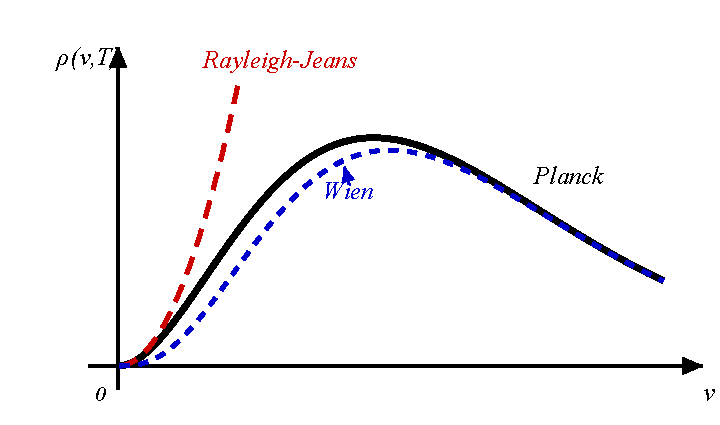
\includegraphics[width=0.72\linewidth]{Capitulo 5/Figuras/EspectroCuerpoNegro.pdf}
                \caption{Densidad espectral de la radiación de un cuerpo negro a temperatura fija. La ley de Rayleigh y Jeans crece sin límite con la frecuencia, la de Wien falla en el infrarrojo, y la de Planck coincide con cada una de ellas en su propio dominio de validez.}
                \label{fig:EspectroCuerpoNegro}
            \end{figure}

            Esta fórmula contiene a las dos que pretendía reconciliar. En el límite de frecuencia baja, sustituyendo \eqref{eq:LimiteBajaFrec},
            \begin{equation}\label{eq:RecuperaRJ}
                \rho \xrightarrow[h\nu\ll k_{B}T]{} \frac{8\pi\nu^{2}}{c^{3}}k_{B}T,
            \end{equation}
            que es exactamente la ley de Rayleigh y Jeans \eqref{eq:RayleighJeans}. En el límite de frecuencia alta, sustituyendo \eqref{eq:LimiteAltaFrec},
            \begin{equation}\label{eq:RecuperaWien}
                \rho \xrightarrow[h\nu\gg k_{B}T]{} \frac{8\pi h\nu^{3}}{c^{3}}\,e^{-h\nu/k_{B}T},
            \end{equation}
            que es la ley de Wien \eqref{eq:LeyWien} con las constantes empíricas identificadas como $\alpha = 8\pi h/c^{3}$ y $\beta = h/k_{B}$. Las dos constantes que Wien había tenido que ajustar a los datos quedan así expresadas en términos de constantes fundamentales, y esa es la primera de las razones por las cuales la fórmula de Planck se impuso de inmediato.

            La segunda razón es que la energía total ya no diverge. Integrando \eqref{eq:LeyPlanck} sobre todas las frecuencias y sustituyendo $y = h\nu/k_{B}T$, de donde $\nu = k_{B}Ty/h$ y $d\nu = k_{B}T\,dy/h$,
            \begin{equation}\label{eq:StefanPaso}
                u(T) = \int_{0}^{\infty}\frac{8\pi h\nu^{3}}{c^{3}}\frac{d\nu}{e^{h\nu/k_{B}T}-1}
                = \frac{8\pi h}{c^{3}}\left(\frac{k_{B}T}{h}\right)^{4}\int_{0}^{\infty}\frac{y^{3}}{e^{y}-1}\,dy,
            \end{equation}
            donde el factor $(k_{B}T/h)^{4}$ proviene de los tres factores del cubo más el que aporta el diferencial. La integral restante es un número puro cuyo valor es $\pi^{4}/15$, de manera que
            \begin{equation}\label{eq:StefanBoltzmann}
                u(T) = \frac{8\pi^{5}k_{B}^{4}}{15c^{3}h^{3}}\,T^{4} \equiv a\,T^{4},
            \end{equation}
            que es la ley que Josef Stefan había establecido experimentalmente en 1879 y que Boltzmann había deducido termodinámicamente en 1884. La ley de Planck no solo cura la divergencia sino que predice el valor numérico de la constante de Stefan a partir de $h$, $c$ y $k_{B}$, y el acuerdo con la medida fue lo que permitió a Planck obtener, en el mismo trabajo de 1900, la primera determinación razonablemente precisa de la constante que hoy lleva su nombre y, a partir de ella, del número de Avogadro y de la carga del electrón, años antes de que Millikan la midiera directamente.

            Queda por señalar la ironía histórica. La ley \eqref{eq:LeyPlanck} es correcta, y su deducción tal como la hemos presentado es esencialmente la que hoy se considera válida, pero la interpretación que Planck le dio no lo era. Él entendía la discretización como una propiedad de los resonadores materiales o incluso como un artificio de cálculo destinado a desaparecer en un tratamiento más fino, y dedicó la década siguiente a intentar deducir su propia fórmula sin recurrir a la hipótesis \ref{sup:Planck}. Nunca lo consiguió, porque no puede conseguirse. Planck abrió la puerta de la física cuántica convencido de que se trataba de una ventana que acabaría cerrándose, y fue Einstein quien, cinco años más tarde, comprendió que lo que había al otro lado era una casa entera.

    \subsection{La cuantización de la radiación según Einstein}

        El artículo que Albert Einstein envió a los \textit{Annalen der Physik} en marzo de 1905, el primero de los cuatro de aquel año prodigioso, lleva un título deliberadamente cauteloso: \textit{Sobre un punto de vista heurístico relativo a la producción y transformación de la luz}. Einstein lo describió en una carta a su amigo Conrad Habicht como el único de los cuatro que era \textit{muy revolucionario}, y tenía razón, porque mientras la relatividad especial modificaba la cinemática sin tocar el carácter ondulatorio de la luz, este trabajo afirmaba que la luz misma tiene estructura granular.

        De entrada hay que decir lo que no es este artículo. No es un trabajo sobre el efecto fotoeléctrico, al que dedica apenas dos páginas de las diecisiete, y no parte de la ley de Planck, de la que Einstein desconfiaba porque su deducción le parecía internamente inconsistente. \textbf{El argumento central es termodinámico y estadístico: Einstein calcula la entropía de la radiación en el régimen de Wien, la compara con la entropía de un gas ideal y demuestra que ambas tienen exactamente la misma dependencia con el volumen, de lo cual concluye que la radiación se comporta, en ese régimen, como si estuviera compuesta de partículas independientes.} Vamos a reproducir ese razonamiento paso a paso.

            Partimos de la ley de Wien \eqref{eq:LeyWien}, que Einstein toma como dato experimental firme en el dominio de frecuencia alta y que no requiere ninguna hipótesis sobre su origen,
            \begin{equation}\label{eq:WienPunto}
                \rho(\nu,T) = \alpha\nu^{3}e^{-\beta\nu/T} .
            \end{equation}
            El primer paso consiste en despejar la temperatura, porque la termodinámica relaciona la entropía con la energía a través de ella. Tomando logaritmos en \eqref{eq:WienPunto},
            \begin{equation}\label{eq:LogWien}
                \ln\rho = \ln\left(\alpha\nu^{3}\right) - \frac{\beta\nu}{T}
                \qquad\Longrightarrow\qquad
                \frac{\beta\nu}{T} = \ln\left(\alpha\nu^{3}\right) - \ln\rho = -\ln\frac{\rho}{\alpha\nu^{3}},
            \end{equation}
            de donde
            \begin{equation}\label{eq:UnoSobreT}
                \frac{1}{T} = -\frac{1}{\beta\nu}\ln\frac{\rho}{\alpha\nu^{3}} .
            \end{equation}

            Introducimos ahora la densidad de entropía espectral $\varphi(\rho,\nu)$, definida de manera que la entropía contenida en un volumen $V$ en el intervalo de frecuencias $d\nu$ sea $V\varphi\,d\nu$. La relación termodinámica fundamental, aplicada a volumen constante, establece que
            \begin{equation}\label{eq:RelacionTermo}
                \frac{\partial\varphi}{\partial\rho} = \frac{1}{T},
            \end{equation}
            de manera que sustituyendo \eqref{eq:UnoSobreT} tenemos una ecuación diferencial para $\varphi$,
            \begin{equation}\label{eq:EDOEntropia}
                \frac{\partial\varphi}{\partial\rho} = -\frac{1}{\beta\nu}\ln\frac{\rho}{\alpha\nu^{3}} .
            \end{equation}
            Integrémosla respecto de $\rho$. Recordando la primitiva $\int\ln(u)\,du = u\ln u - u$, y tratando $\nu$ como un parámetro,
            \begin{equation}\label{eq:IntegralEntropia}
                \varphi = -\frac{1}{\beta\nu}\int\ln\frac{\rho}{\alpha\nu^{3}}\,d\rho
                = -\frac{\rho}{\beta\nu}\left[\ln\frac{\rho}{\alpha\nu^{3}} - 1\right],
            \end{equation}
            donde la constante de integración se fija a cero exigiendo que la entropía se anule con la densidad de energía.

            Consideremos ahora una cantidad total de energía $E$ contenida en el volumen $V$, en el intervalo de frecuencias entre $\nu$ y $\nu + d\nu$, de manera que la densidad espectral es
            \begin{equation}\label{eq:RhoDeE}
                \rho = \frac{E}{V\,d\nu} .
            \end{equation}
            La entropía total de esa radiación es $S = V\varphi\,d\nu$, y sustituyendo \eqref{eq:IntegralEntropia} y \eqref{eq:RhoDeE},
            \begin{equation}\label{eq:EntropiaTotal}
                S = V\,d\nu\left(-\frac{E}{V\,d\nu\,\beta\nu}\right)\left[\ln\frac{E}{V\,d\nu\,\alpha\nu^{3}} - 1\right]
                = -\frac{E}{\beta\nu}\left[\ln\frac{E}{V\alpha\nu^{3}d\nu} - 1\right],
            \end{equation}
            donde el factor $V\,d\nu$ se ha cancelado con el que aparece en el denominador de la fracción exterior.

            Aquí llega el paso decisivo, y es de una sencillez desarmante. Preguntémonos cómo cambia esta entropía cuando la misma energía $E$ ocupa un volumen distinto, manteniendo fija la frecuencia. Escribiendo \eqref{eq:EntropiaTotal} para dos volúmenes $V$ y $V_{0}$ y restando,
            \begin{equation}\label{eq:DiferenciaEntropia1}
                S - S_{0} = -\frac{E}{\beta\nu}\left[\ln\frac{E}{V\alpha\nu^{3}d\nu} - \textcolor{red}{1} - \ln\frac{E}{V_{0}\alpha\nu^{3}d\nu} + \textcolor{red}{1}\right],
            \end{equation}
            donde los dos unos marcados en rojo se cancelan. La diferencia de logaritmos es el logaritmo del cociente, y en ese cociente se cancelan todos los factores comunes, es decir, $E$, $\alpha$, $\nu^{3}$ y $d\nu$, sobreviviendo únicamente los volúmenes,
            \begin{equation}\label{eq:DiferenciaEntropia2}
                S - S_{0} = -\frac{E}{\beta\nu}\ln\frac{V_{0}}{V} = \frac{E}{\beta\nu}\ln\frac{V}{V_{0}} .
            \end{equation}

            La expresión \eqref{eq:DiferenciaEntropia2} es el corazón del artículo de 1905, y su forma debió resultarle a Einstein inmediatamente reconocible, porque es idéntica a la que gobierna la expansión isoterma de un gas ideal.

            Consideremos, en efecto, un gas de $n$ partículas independientes encerradas en un volumen $V_{0}$, y preguntémonos cuál es la probabilidad de que en un instante dado todas ellas se encuentren simultáneamente dentro de una subregión de volumen $V$. Para una sola partícula, y suponiendo que su posición es uniformemente aleatoria, esa probabilidad es simplemente la razón de volúmenes $V/V_{0}$. Como las partículas son independientes, las probabilidades se multiplican, de manera que
            \begin{equation}\label{eq:ProbabilidadGas}
                W = \left(\frac{V}{V_{0}}\right)^{n} .
            \end{equation}
            El principio de Boltzmann, que Einstein escribe en la forma $S - S_{0} = k_{B}\ln W$ y que él mismo consideraba la relación más importante de toda la física estadística, da entonces
            \begin{equation}\label{eq:BoltzmannGas}
                S - S_{0} = k_{B}\ln\left(\frac{V}{V_{0}}\right)^{n} = n\,k_{B}\ln\frac{V}{V_{0}} .
            \end{equation}

            Al comparar \eqref{eq:DiferenciaEntropia2}, que se refiere a radiación, con \eqref{eq:BoltzmannGas}, que se refiere a un gas de partículas, se ve que ambas son proporcionales al logaritmo del cociente de volúmenes, y que la constante de proporcionalidad es $E/\beta\nu$ en un caso y $nk_{B}$ en el otro. Igualándolas,
            \begin{equation}\label{eq:IgualacionEinstein}
                \frac{E}{\beta\nu} = n\,k_{B}
                \qquad\Longrightarrow\qquad
                E = n\,k_{B}\beta\,\nu .
            \end{equation}
            Recordando que la constante $\beta$ de la ley de Wien vale $\beta = h/k_{B}$, según identificamos en \eqref{eq:RecuperaWien} al comparar con la ley de Planck, el producto $k_{B}\beta$ es exactamente $h$ y por tanto
            \begin{equation}\label{eq:ResultadoEinstein}
                \boxed{\;E = n\,h\nu .\;}
            \end{equation}

            Hay que ser muy preciso sobre lo que este cálculo demuestra y lo que no. No demuestra que la luz esté hecha de partículas en el sentido de pequeñas bolas que viajan por el espacio; demuestra que la entropía de la radiación monocromática, en el régimen de validez de la ley de Wien, depende del volumen exactamente como lo haría la de un gas de $n = E/h\nu$ entidades independientes. Einstein lo formuló con esa misma cautela en el enunciado que cierra su sección sexta: la radiación se comporta, desde el punto de vista termodinámico, \textit{como si} estuviera constituida por cuantos de energía independientes de magnitud $h\nu$. Que la conclusión sea estadística y no mecánica no la debilita; al contrario, la hace más robusta, porque no depende de ningún modelo sobre la estructura interna de esos cuantos.

            Dos observaciones completan el argumento. La primera es que la independencia mutua de los cuantos, que es lo que permite multiplicar las probabilidades en \eqref{eq:ProbabilidadGas}, solo se cumple en el régimen de Wien, es decir, cuando $h\nu\gg k_{B}T$ y el número de ocupación de cada modo es muy pequeño; en el régimen de Rayleigh y Jeans los cuantos no son independientes, y esa correlación, que Einstein analizó en 1909 al estudiar las fluctuaciones de energía de la radiación, es el primer indicio de lo que hoy llamamos estadística de Bose y del agrupamiento de fotones que Hanbury Brown y Twiss medirían medio siglo después. La segunda es que el paso de Planck a Einstein es un salto genuino y no una reformulación: Planck había cuantizado el intercambio de energía entre la materia y el campo, mientras que Einstein cuantiza el campo libre mismo, que puede propagarse durante millones de años a través del espacio vacío sin dejar de estar constituido por cuantos.

            Habiendo establecido la hipótesis, Einstein dedica las últimas páginas del artículo a extraer de ella consecuencias susceptibles de contraste experimental, y presenta tres.

            La primera es la regla de Stokes para la fotoluminiscencia, según la cual la luz reemitida por una sustancia fluorescente tiene siempre una frecuencia menor o igual que la de la luz incidente. En el marco clásico esta regla es un hecho empírico sin explicación; en el de Einstein es inmediata, pues un cuanto incidente de energía $h\nu$ no puede producir un cuanto emitido de energía mayor, ya que ello violaría la conservación de la energía en el proceso elemental,
            \begin{equation}\label{eq:Stokes}
                h\nu_{\text{emitido}} \leq h\nu_{\text{incidente}}
                \qquad\Longrightarrow\qquad
                \nu_{\text{emitido}} \leq \nu_{\text{incidente}} .
            \end{equation}

            La segunda es el efecto fotoeléctrico, descubierto por Hertz en 1887 de manera accidental mientras verificaba la existencia de las ondas de Maxwell y estudiado sistemáticamente por Lenard en 1902. El fenómeno consiste en que la luz que incide sobre un metal arranca electrones, y presenta tres rasgos que la teoría ondulatoria no puede explicar. El primero es la existencia de una frecuencia umbral por debajo de la cual no se emite ningún electrón por intensa que sea la iluminación, mientras que clásicamente una onda de intensidad suficiente debería acabar arrancándolos siempre. El segundo es que la energía de los electrones emitidos no depende de la intensidad sino de la frecuencia, cuando clásicamente la energía transportada por la onda es proporcional al cuadrado de la amplitud y por tanto a la intensidad. El tercero es la instantaneidad del proceso, pues los electrones aparecen sin retardo apreciable, mientras que un cálculo clásico del tiempo que tardaría un electrón en acumular la energía necesaria a partir de una onda débil arroja intervalos de minutos o de horas.

            La explicación de Einstein cabe en una línea. Si la luz consiste en cuantos de energía $h\nu$ y cada electrón absorbe uno solo de ellos, entonces la energía disponible para el electrón es $h\nu$, de la cual debe invertir una cantidad $W$, característica del metal y llamada \textit{función de trabajo}, en escapar de la superficie. La energía cinética máxima con que puede salir es, por tanto,
            \begin{equation}\label{eq:Fotoelectrico}
                \boxed{\;E_{\text{cin}}^{\max} = h\nu - W .\;}
            \end{equation}
            Las tres anomalías quedan explicadas simultáneamente. Existe una frecuencia umbral $\nu_{0} = W/h$ porque por debajo de ella el miembro derecho de \eqref{eq:Fotoelectrico} es negativo y el electrón no puede escapar; la energía depende de la frecuencia y no de la intensidad porque cada electrón interactúa con un solo cuanto, y aumentar la intensidad significa aumentar el número de cuantos y por tanto el número de electrones emitidos, no su energía individual; y el proceso es instantáneo porque no hay nada que acumular, ya que la transferencia ocurre de golpe.

            La predicción cuantitativa contenida en \eqref{eq:Fotoelectrico} es especialmente exigente y merece subrayarse, porque es la que decidió el asunto. Si se mide el potencial de frenado $V_{s}$ necesario para detener a los electrones más energéticos, se tiene $eV_{s} = E_{\text{cin}}^{\max}$ y por tanto
            \begin{equation}\label{eq:PotencialFrenado}
                V_{s} = \frac{h}{e}\,\nu - \frac{W}{e},
            \end{equation}
            de manera que al representar $V_{s}$ frente a $\nu$, como en la figura \ref{fig:Fotoelectrico}, debe obtenerse una recta cuya pendiente es $h/e$ y por tanto la misma para todos los metales, variando únicamente la ordenada en el origen. Robert Millikan dedicó diez años a intentar refutar esta predicción, en la que no creía, y en 1916 publicó la medida más cuidadosa que se había hecho del efecto, obteniendo rectas perfectas con una pendiente que daba $h = 6{,}57\times 10^{-34}\,\mathrm{J\,s}$, en excelente acuerdo con el valor deducido por Planck del espectro del cuerpo negro por un camino completamente distinto. Millikan reconoció que la ecuación de Einstein describía los datos con exactitud, pero siguió rechazando la hipótesis de los cuantos de luz que la sustentaba, lo cual ilustra hasta qué punto resultaba difícil de aceptar. El premio Nobel de 1921 le fue concedido a Einstein, de manera explícita, por el descubrimiento de la ley del efecto fotoeléctrico y no por la relatividad.

            \begin{figure}[htbp]
                \centering
                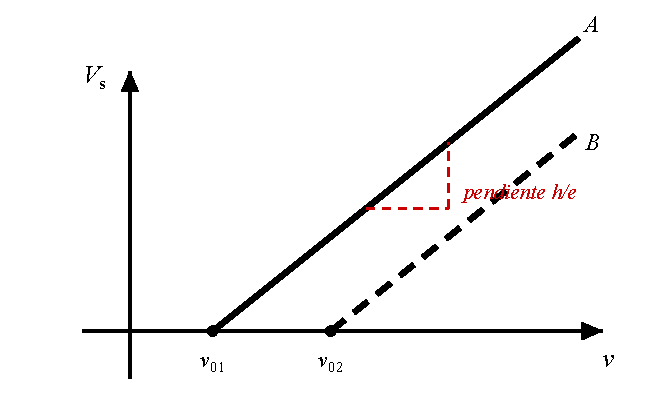
\includegraphics[width=0.62\linewidth]{Capitulo 5/Figuras/Fotoelectrico.pdf}
                \caption{Potencial de frenado frente a la frecuencia de la luz incidente para dos metales distintos. La predicción de Einstein es que las dos rectas sean paralelas, con pendiente $h/e$ común, y que solo difieran en la frecuencia umbral.}
                \label{fig:Fotoelectrico}
            \end{figure}

            La tercera consecuencia es la fotoionización, para la cual Einstein predice que la energía del cuanto debe ser al menos igual al potencial de ionización de la molécula, prediciendo también aquí un umbral en frecuencia.

    \subsection{El momento del cuanto: de Einstein 1917 al efecto Compton}

        Las tres consecuencias anteriores se refieren únicamente a la energía del cuanto. Un cuanto de luz con estructura de partícula debería poseer además \textit{momento lineal}, y esa segunda mitad del argumento tardó doce años en llegar y otros seis en comprobarse.

            En 1917 Einstein volvió sobre el problema del cuerpo negro con un artículo, \textit{Zur Quantentheorie der Strahlung}, que contiene dos aportaciones mayores. La primera es una deducción nueva y mucho más transparente de la ley de Planck, basada en el equilibrio detallado entre la materia y la radiación. Einstein considera moléculas con dos niveles de energía $\epsilon_{n}$ y $\epsilon_{m}$, con $\epsilon_{m}>\epsilon_{n}$, y postula tres procesos elementales: la absorción, con probabilidad proporcional a la densidad de radiación y coeficiente $B_{nm}$; la emisión estimulada por la radiación, con coeficiente $B_{mn}$; y la \textit{emisión espontánea}, con coeficiente $A_{mn}$, que ocurre sin necesidad de campo externo y que Einstein introduce por primera vez en este trabajo. En equilibrio, el número de transiciones en cada sentido debe igualarse,
            \begin{equation}\label{eq:BalanceDetallado}
                N_{n}B_{nm}\,\rho = N_{m}\left(B_{mn}\,\rho + A_{mn}\right),
            \end{equation}
            y usando la distribución de Boltzmann para las poblaciones, $N_{m}/N_{n} = e^{-(\epsilon_{m}-\epsilon_{n})/k_{B}T}$, se despeja la densidad espectral,
            \begin{equation}\label{eq:DespejeRho}
                \rho = \frac{A_{mn}/B_{mn}}{\dfrac{B_{nm}}{B_{mn}}e^{(\epsilon_{m}-\epsilon_{n})/k_{B}T} - 1} .
            \end{equation}
            Exigiendo que \eqref{eq:DespejeRho} se reduzca a la ley de Rayleigh y Jeans a temperatura muy alta se obtiene $B_{nm} = B_{mn}$, y comparando con la ley de Planck \eqref{eq:LeyPlanck} se obtienen de golpe las dos relaciones
            \begin{equation}\label{eq:RelacionesAB}
                \epsilon_{m}-\epsilon_{n} = h\nu
                \qquad\text{y}\qquad
                \frac{A_{mn}}{B_{mn}} = \frac{8\pi h\nu^{3}}{c^{3}} .
            \end{equation}
            La primera es la segunda regla de Bohr, que aquí no se postula sino que se deduce; la segunda fija la razón entre emisión espontánea y estimulada y es, cuarenta y tres años antes de Maiman, el fundamento teórico del láser, cuyo funcionamiento consiste precisamente en conseguir que la emisión estimulada domine sobre la espontánea mediante una inversión de población.

            La segunda aportación del artículo es la que aquí nos interesa. Einstein demuestra que para que las moléculas en equilibrio con la radiación de Planck mantengan la distribución de velocidades de Maxwell, no basta con contabilizar el intercambio de energía: hay que contabilizar también el intercambio de \textit{momento}, y los procesos elementales deben ser \textit{direccionales}. Si una molécula emite una energía $h\nu$, debe retroceder con un momento
            \begin{equation}\label{eq:MomentoCuanto}
                p = \frac{h\nu}{c} = \frac{h}{\lambda} = \hbar k,
            \end{equation}
            en una dirección bien definida, y no emitir una onda esférica que no produciría retroceso neto alguno. La conclusión de Einstein es tajante: la radiación saliente en forma de ondas esféricas no existe en los procesos elementales. Lo que llamamos onda esférica es la distribución de probabilidad de la dirección de emisión, no la emisión misma.

            El propio Einstein señala la incomodidad que le producía el resultado, en una frase que anticipa medio siglo de debate: \textit{la debilidad de la teoría radica en que deja la duración y la dirección de los procesos elementales al azar; no obstante, confío plenamente en que el camino elegido es el correcto}. La aleatoriedad que le incomodaba resultó ser irreducible, y la emisión espontánea que él tuvo que postular quedó explicada diez años más tarde por Dirac como emisión estimulada por las fluctuaciones del vacío que calcularemos más adelante en este capítulo.

            La comprobación directa de \eqref{eq:MomentoCuanto} llegó en 1923 de la mano de Arthur Compton, y fue el experimento que finalmente convenció a la comunidad. Compton hizo incidir rayos X de longitud de onda $\lambda$ sobre un blanco de grafito y midió la longitud de onda de la radiación dispersada en función del ángulo, encontrando que era \textit{mayor} que la incidente. Clásicamente esto es imposible: una onda electromagnética hace oscilar a los electrones a su propia frecuencia y estos reemiten a esa misma frecuencia, de manera que la longitud de onda no puede cambiar. Si en cambio la radiación consiste en cuantos con energía $h\nu$ y momento $h\nu/c$, el proceso es una colisión elástica entre dos partículas y el cuanto debe ceder parte de su energía al electrón, saliendo con menor frecuencia.

            \begin{figure}[htbp]
                \centering
                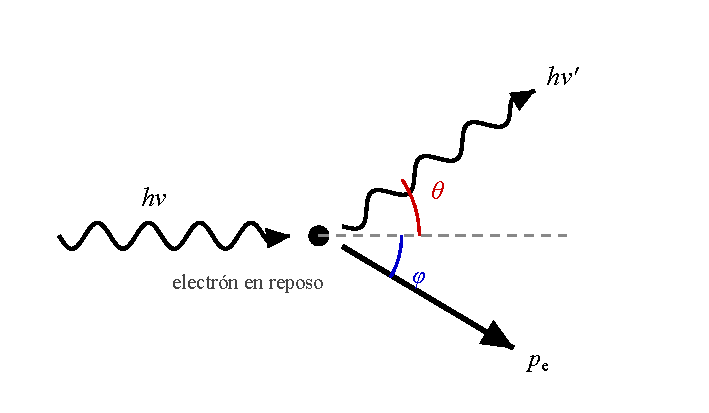
\includegraphics[width=0.72\linewidth]{Capitulo 5/Figuras/Compton.pdf}
                \caption{Geometría de la dispersión de Compton. El cuanto incidente cede parte de su energía y de su momento al electrón, que retrocede, y sale con una frecuencia menor y desviado un ángulo $\theta$.}
                \label{fig:Compton}
            \end{figure}

            El cálculo completo es un ejercicio de cinemática relativista. Sea un cuanto de frecuencia $\nu$ que incide sobre un electrón en reposo, de masa $m_{e}$, y que tras la colisión sale con frecuencia $\nu'$ formando un ángulo $\theta$ con la dirección incidente, mientras el electrón retrocede con momento $\mathbf{p}_{e}$ formando un ángulo $\varphi$ al otro lado, según la geometría de la figura \ref{fig:Compton}. La conservación del momento, proyectada sobre la dirección incidente y sobre la perpendicular, da
            \begin{align}
                \frac{h\nu}{c} &= \frac{h\nu'}{c}\cos\theta + p_{e}\cos\varphi, \label{eq:ComptonPx}\\
                0 &= \frac{h\nu'}{c}\sin\theta - p_{e}\sin\varphi, \label{eq:ComptonPy}
            \end{align}
            y la conservación de la energía, usando la expresión relativista para el electrón,
            \begin{equation}\label{eq:ComptonE}
                h\nu + m_{e}c^{2} = h\nu' + \sqrt{p_{e}^{2}c^{2}+m_{e}^{2}c^{4}} .
            \end{equation}

            El ángulo $\varphi$ del electrón no interesa, así que lo eliminamos. Despejando los términos que lo contienen en \eqref{eq:ComptonPx} y \eqref{eq:ComptonPy},
            \begin{equation}\label{eq:ComptonDespeje}
                p_{e}\cos\varphi = \frac{h\nu}{c} - \frac{h\nu'}{c}\cos\theta,
                \qquad
                p_{e}\sin\varphi = \frac{h\nu'}{c}\sin\theta,
            \end{equation}
            elevando ambas al cuadrado y sumándolas, con lo cual el miembro izquierdo se convierte en $p_{e}^{2}$ gracias a la identidad pitagórica,
            \begin{equation}\label{eq:ComptonSuma}
                p_{e}^{2} = \frac{h^{2}\nu^{2}}{c^{2}} - \frac{2h^{2}\nu\nu'}{c^{2}}\cos\theta + \frac{h^{2}\nu'^{2}}{c^{2}}\cos^{2}\theta + \frac{h^{2}\nu'^{2}}{c^{2}}\sin^{2}\theta,
            \end{equation}
            y usando de nuevo $\cos^{2}\theta+\sin^{2}\theta = 1$ para reunir los dos últimos términos,
            \begin{equation}\label{eq:ComptonPe2}
                p_{e}^{2}c^{2} = h^{2}\nu^{2} + h^{2}\nu'^{2} - 2h^{2}\nu\nu'\cos\theta .
            \end{equation}

            Trabajemos ahora la ecuación de la energía. Pasando $h\nu'$ al miembro izquierdo de \eqref{eq:ComptonE} y elevando al cuadrado para eliminar la raíz,
            \begin{equation}\label{eq:ComptonECuadrado}
                \left[h\left(\nu-\nu'\right) + m_{e}c^{2}\right]^{2} = p_{e}^{2}c^{2} + m_{e}^{2}c^{4},
            \end{equation}
            y desarrollando el cuadrado del binomio del miembro izquierdo,
            \begin{equation}\label{eq:ComptonDesarrollo}
                h^{2}\left(\nu-\nu'\right)^{2} + 2h\left(\nu-\nu'\right)m_{e}c^{2} + \textcolor{red}{m_{e}^{2}c^{4}} = p_{e}^{2}c^{2} + \textcolor{red}{m_{e}^{2}c^{4}},
            \end{equation}
            donde los dos términos marcados en rojo son idénticos y se cancelan. Desarrollando además el primer cuadrado,
            \begin{equation}\label{eq:ComptonPe2bis}
                p_{e}^{2}c^{2} = h^{2}\nu^{2} - 2h^{2}\nu\nu' + h^{2}\nu'^{2} + 2h\left(\nu-\nu'\right)m_{e}c^{2} .
            \end{equation}

            Tenemos ahora dos expresiones para la misma cantidad, \eqref{eq:ComptonPe2} y \eqref{eq:ComptonPe2bis}. Igualándolas, los términos $h^{2}\nu^{2}$ y $h^{2}\nu'^{2}$ aparecen en ambos miembros y se cancelan,
            \begin{equation}\label{eq:ComptonIgualacion}
                \textcolor{red}{h^{2}\nu^{2}} + \textcolor{red}{h^{2}\nu'^{2}} - 2h^{2}\nu\nu'\cos\theta = \textcolor{red}{h^{2}\nu^{2}} + \textcolor{red}{h^{2}\nu'^{2}} - 2h^{2}\nu\nu' + 2h\left(\nu-\nu'\right)m_{e}c^{2},
            \end{equation}
            y lo que queda, tras dividir todo por $2h$, es
            \begin{equation}\label{eq:ComptonCasi}
                -h\nu\nu'\cos\theta = -h\nu\nu' + \left(\nu-\nu'\right)m_{e}c^{2}
                \qquad\Longrightarrow\qquad
                h\nu\nu'\left(1-\cos\theta\right) = \left(\nu-\nu'\right)m_{e}c^{2} .
            \end{equation}
            Dividiendo ambos miembros por $\nu\nu'm_{e}c^{2}$,
            \begin{equation}\label{eq:ComptonFrecuencias}
                \frac{h}{m_{e}c^{2}}\left(1-\cos\theta\right) = \frac{\nu-\nu'}{\nu\nu'} = \frac{1}{\nu'} - \frac{1}{\nu},
            \end{equation}
            y multiplicando por $c$ para pasar de frecuencias a longitudes de onda, con $\lambda = c/\nu$,
            \begin{equation}\label{eq:Compton}
                \boxed{\;\Delta\lambda = \lambda' - \lambda = \frac{h}{m_{e}c}\left(1-\cos\theta\right) .\;}
            \end{equation}

            La fórmula \eqref{eq:Compton} tiene tres rasgos que la convierten en una prueba demoledora. El primero es que el corrimiento no depende de la longitud de onda incidente ni del material del blanco, sino únicamente del ángulo de observación, lo cual es una predicción rígida sin ningún parámetro ajustable. El segundo es que la constante que fija la escala,
            \begin{equation}\label{eq:LongitudCompton}
                \lambda_{C} = \frac{h}{m_{e}c} = 2{,}426\times 10^{-12}\,\mathrm{m},
            \end{equation}
            llamada \textit{longitud de onda de Compton del electrón}, combina la constante de Planck con la masa del electrón y la velocidad de la luz, de manera que medir la pendiente del corrimiento frente a $1-\cos\theta$ equivale a medir $h$ por un tercer camino independiente, y el valor obtenido coincidió con los de Planck y Millikan. El tercero es que el efecto es despreciable para luz visible, donde $\lambda_{C}/\lambda \sim 10^{-6}$, y solo se hace visible con rayos X, lo cual explica por qué nadie lo había observado antes.

            La comunidad se rindió ante este resultado, y no es difícil ver por qué. El efecto Compton es el experimento que cerró el debate, porque a diferencia del efecto fotoeléctrico, que admitía explicaciones semiclásicas alternativas en las que el campo permanecía continuo y era el átomo el que estaba cuantizado, aquí lo que se observa es una colisión entre dos objetos con energía y momento bien definidos. Compton recibió el premio Nobel en 1927, el mismo año en que Dirac cuantizó el campo electromagnético, y la palabra \textit{fotón}, acuñada por el químico Gilbert Lewis en 1926 para designar una entidad bastante distinta de la que hoy nombra, se impuso precisamente en esos años.

    \subsection{El fotón es indivisible: el experimento de Grangier, Roger y Aspect}

        Los argumentos anteriores establecen que la luz intercambia energía y momento en unidades discretas, pero ninguno de ellos obliga estrictamente a cuantizar el campo. Existe una escapatoria, y durante décadas hubo quien la defendió: se puede mantener un campo electromagnético clásico y continuo, y atribuir toda la discreción a la materia, es decir, a los átomos y a los detectores, que están cuantizados y por tanto solo pueden absorber energía en paquetes. Esta descripción, llamada \textit{semiclásica}, reproduce correctamente el efecto fotoeléctrico, el efecto Compton en su versión no relativista y buena parte de la óptica. Para demostrar que el campo mismo está cuantizado hace falta un experimento en el cual la predicción semiclásica y la cuántica difieran, y ese experimento tuvo que esperar hasta 1986.

            La idea es muy simple. Enviemos luz muy débil sobre un divisor de haz equilibrado, con un detector en cada salida, y preguntémonos con qué frecuencia ambos detectores se disparan a la vez. Una onda clásica, por débil que sea, se divide: una mitad se transmite y la otra se refleja, de manera que ambos detectores reciben señal simultáneamente y las coincidencias son frecuentes. Una partícula indivisible, en cambio, toma un camino o el otro y jamás los dos, de manera que las coincidencias deberían desaparecer por completo.

            Este argumento cualitativo se cuantifica mediante el \textit{parámetro de anticorrelación}
            \begin{equation}\label{eq:ParametroAlpha}
                \alpha \equiv \frac{P_{c}}{P_{t}\,P_{r}},
            \end{equation}
            donde $P_{t}$ y $P_{r}$ son las probabilidades de detección en los brazos transmitido y reflejado y $P_{c}$ la probabilidad de detección conjunta. Si las dos detecciones fuesen sucesos estadísticamente independientes se tendría $P_{c} = P_{t}P_{r}$ y por tanto $\alpha = 1$.

            El punto clave es el siguiente: cualquier teoría en la cual el campo sea una onda clásica, incluso si se le permite fluctuar aleatoriamente de la manera más caprichosa, predice
            \begin{equation}\label{eq:DesigualdadClasica}
                \alpha \geq 1 .
            \end{equation}
            La demostración se sigue de la desigualdad de Cauchy y Schwarz. En una descripción clásica, las probabilidades de detección son proporcionales a la intensidad instantánea $I(t)$ en cada brazo, y para un divisor equilibrado ambas son iguales a $I/2$; promediando sobre las fluctuaciones de la fuente, $P_{t} = P_{r} = \eta\overline{I}/2$ y $P_{c} = \eta^{2}\overline{I^{2}}/4$, de donde
            \begin{equation}\label{eq:AlphaClasico}
                \alpha = \frac{\eta^{2}\overline{I^{2}}/4}{\eta^{2}\overline{I}^{2}/4} = \frac{\overline{I^{2}}}{\overline{I}^{\,2}} \geq 1,
            \end{equation}
            porque la varianza $\overline{I^{2}} - \overline{I}^{\,2}$ de una cantidad real es siempre no negativa. La desigualdad \eqref{eq:AlphaClasico} no depende de ningún modelo concreto de la fuente: vale para cualquier distribución de intensidades positiva, y por tanto para toda teoría ondulatoria clásica imaginable. La teoría cuántica, en cambio, predice $\alpha = 0$ para un estado de un solo fotón, pues un único cuanto no puede ser detectado dos veces.

            El problema práctico es preparar un estado con \textit{un solo} fotón. Atenuar un láser no sirve, porque un haz coherente muy débil sigue siendo una superposición de estados de distinto número de fotones con estadística de Poisson, y para ella $\alpha = 1$ exactamente, indistinguible del límite clásico. Philippe Grangier, Gérard Roger y Alain Aspect resolvieron el problema en el Instituto de Óptica de Orsay recurriendo a una \textit{cascada radiativa atómica} \citep{Alan-Aspect}.

            La fuente es un haz atómico de calcio 40 excitado selectivamente por dos láseres hasta el nivel $4p^{2}\,{}^{1}S_{0}$. Desde allí el átomo decae en dos etapas sucesivas, emitiendo primero un fotón $\nu_{1}$ de $551{,}3$ nm, en el verde, al pasar al nivel intermedio $4s4p\,{}^{1}P_{1}$, y a continuación un segundo fotón $\nu_{2}$ de $422{,}7$ nm, en el violeta, al volver al fundamental $4s^{2}\,{}^{1}S_{0}$. La vida media del nivel intermedio es de unos $4{,}7$ ns, muy corta comparada con el intervalo medio entre cascadas sucesivas, que se ajusta mediante la densidad del haz atómico.

            El truco consiste en usar el primer fotón como \textit{heraldo}. La detección de $\nu_{1}$ en un fotomultiplicador, filtrado espectralmente para que solo acepte el verde, indica que el átomo se encuentra en el nivel intermedio y que por tanto se emitirá un fotón violeta en los próximos nanosegundos. Esa detección abre una ventana temporal electrónica de duración $w\approx 9$ ns durante la cual se observa el segundo canal. Dentro de esa ventana, y solo dentro de ella, se tiene la certeza de que el campo violeta contiene exactamente un fotón, que es precisamente el estado que ninguna fuente atenuada puede proporcionar.

            El fotón $\nu_{2}$ así preparado incide sobre un divisor de haz equilibrado, con un fotomultiplicador en la salida transmitida y otro en la reflejada, y un circuito de coincidencias registra las detecciones conjuntas dentro de la ventana. El esquema completo se muestra en la figura \ref{fig:Aspect}. En estas condiciones el parámetro \eqref{eq:ParametroAlpha} se determina a partir de los conteos medidos como
            \begin{equation}\label{eq:AlphaMedido}
                \alpha = \frac{N_{c}\,N_{1}}{N_{t}\,N_{r}},
            \end{equation}
            donde $N_{1}$ es el número de disparos del detector heraldo, $N_{t}$ y $N_{r}$ los de coincidencias dobles entre el heraldo y cada brazo, y $N_{c}$ el de coincidencias triples.

            \begin{figure}[htbp]
                \centering
                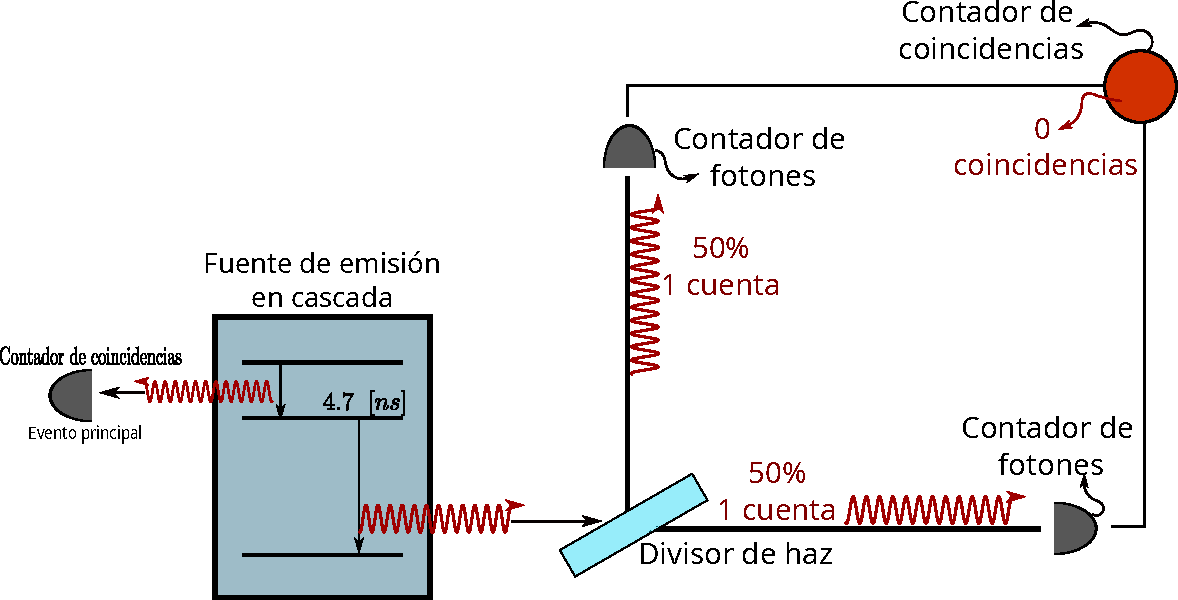
\includegraphics[width=0.9\linewidth]{Capitulo 5/Figuras/Aspect.pdf}
                \caption{Esquema experimental del estudio efectuado por Philippe Grangier, Gérard Roger y Alain Aspect en 1986. La detección del primer fotón de la cascada abre una ventana temporal durante la cual el segundo fotón, preparado en un estado de un solo cuanto, incide sobre un divisor de haz equilibrado con un detector en cada salida.}
                \label{fig:Aspect}
            \end{figure}

            La medida arrojó
            \begin{equation}\label{eq:ResultadoAspect}
                \alpha = 0{,}18 \pm 0{,}06,
            \end{equation}
            es decir, un valor que viola la cota clásica \eqref{eq:DesigualdadClasica} por trece desviaciones estándar. La desviación respecto del cero que predice la teoría cuántica ideal se explica por completo por las cascadas accidentales, esto es, por la probabilidad no nula de que un segundo átomo emita durante la ventana abierta por el primero, y en efecto el valor medido de $\alpha$ disminuye al reducir la duración de la ventana o la densidad del haz, tal como la teoría cuántica predice.

            El peso del argumento está en que no se trata de que el modelo ondulatorio ajuste peor los datos, sino de que \textbf{ninguna teoría en la que la luz sea una onda clásica, por complicada que sea su descripción estadística, puede producir un valor de $\alpha$ menor que uno}, porque ello exigiría que la varianza de una cantidad real fuese negativa. El experimento no refuta un modelo particular sino una clase entera de modelos, y esa es la razón por la cual es concluyente.

            El mismo trabajo contiene una segunda parte igual de importante y menos citada. Los autores tomaron exactamente la misma fuente de fotones individuales y, en lugar del divisor con dos detectores, la enviaron a un interferómetro de Mach y Zehnder, es decir, un montaje en el cual los dos caminos vuelven a recombinarse. Al variar la diferencia de camino observaron franjas de interferencia con una visibilidad del $98\%$. \textbf{El mismo objeto que en el primer montaje se niega tajantemente a dividirse en el divisor de haz, produce en el segundo un patrón de interferencia que exige que haya pasado por los dos brazos a la vez.} Esta es la formulación experimental más limpia que existe de la complementariedad de Bohr: no hay contradicción porque ambos comportamientos nunca se manifiestan en el mismo montaje, y cuál de los dos se observa depende de lo que el experimentador decida medir.

            Una advertencia final para evitar una confusión frecuente. El nombre de Alain Aspect se asocia habitualmente a los experimentos de 1981 y 1982 sobre las desigualdades de Bell, realizados con la misma fuente de cascada de calcio y por los que compartió el premio Nobel de 2022 con John Clauser y Anton Zeilinger; aquellos experimentos midieron correlaciones de polarización entre los dos fotones de la cascada y refutaron las teorías de variables ocultas locales. El experimento que hemos descrito aquí es posterior, de 1986, y su objeto es distinto: no la localidad, sino el carácter indivisible del cuanto de luz. Hay que mantenerlos separados porque responden a preguntas diferentes, aunque ambos usen la misma fuente y el mismo laboratorio.

            Con este resultado queda establecido lo que el título de esta sección anunciaba. La luz intercambia energía en cuantos, transporta momento en cuantos, y no puede dividirse por debajo del cuanto. Lo que resta del capítulo consiste en construir el formalismo que da cuenta de todo ello, y que no consiste en añadir partículas a la teoría electromagnética sino en cuantizar el propio campo, es decir, en aplicar al campo de Maxwell el mismo procedimiento canónico que el capítulo anterior aplicó a una partícula.

\section{Primera y segunda cuantización}

    La física del siglo XX nos legó dos revoluciones conceptuales que transformaron nuestra comprensión de la naturaleza: la mecánica cuántica y la teoría de campos. La óptica cuántica representa la confluencia de ambas tradiciones, aplicando el formalismo de la teoría cuántica de campos al caso particular de la radiación electromagnética. Antes de desarrollar ese formalismo hay que detenerse en qué significa exactamente cuantizar un sistema físico, porque la expresión \textit{segunda cuantización} es, con toda probabilidad, la más desafortunada del vocabulario de la física, y la confusión que genera vale la pena desarmarla de entrada.

    \subsection{Qué cuantiza la primera cuantización}

        El capítulo anterior desarrolló en detalle el procedimiento canónico. Se parte de un sistema mecánico clásico descrito por variables canónicas $q$ y $p$ que satisfacen el corchete de Poisson $\{q_{i},p_{j}\}=\delta_{ij}$, y se las promueve a operadores sobre un espacio de Hilbert sujetos a la relación de conmutación
        \begin{equation}\label{eq:PrimeraCuantizacion}
            \left[\hat{q}_{i},\hat{p}_{j}\right] = i\hbar\,\delta_{ij},
        \end{equation}
        que se obtiene del corchete clásico mediante la correspondencia de Dirac \cite{Dirac1930}. El objeto que resulta de este procedimiento es la función de onda $\psi(\mathbf{r},t)$, cuyo módulo al cuadrado da la densidad de probabilidad de hallar la partícula en cada punto.

        Seamos exactos sobre lo que se ha cuantizado aquí, porque el nombre induce a error. \textbf{Lo que la primera cuantización discretiza no es la posición ni el momento, que siguen teniendo espectro continuo, sino ciertas cantidades como la energía o el momento angular, y solo cuando las condiciones de frontera lo imponen.} Lo que realmente ocurre en \eqref{eq:PrimeraCuantizacion} es que las variables dinámicas dejan de ser números y pasan a ser operadores que no conmutan; la aparición de espectros discretos es una consecuencia de ese cambio de estatuto, no su definición. Un electrón libre, cuantizado en este sentido, tiene energía continua.

        La limitación decisiva del esquema es de otra índole y es puramente estructural: \textbf{el número de partículas es un dato fijo del problema y no una variable dinámica}. La función de onda de una partícula vive en $L^{2}(\mathbb{R}^{3})$, la de dos partículas en $L^{2}(\mathbb{R}^{6})$, y no existe ninguna operación dentro del formalismo que conecte ambos espacios. Si empezamos con una partícula, siempre tendremos una. Para la materia ordinaria a bajas energías esta restricción no molesta, porque los electrones de un átomo ni se crean ni se destruyen, pero para la luz es fatal: los fotones aparecen cuando un átomo emite y desaparecen cuando absorbe, de manera que el número de fotones es precisamente la variable que queremos describir.

    \subsection{Qué cuantiza la segunda cuantización}

        La segunda cuantización no consiste en cuantizar dos veces, y ahí está el origen de toda la confusión. \textbf{Se trata de aplicar el mismo y único procedimiento canónico \eqref{eq:PrimeraCuantizacion}, pero a un objeto distinto: no a las coordenadas de una partícula, sino a los grados de libertad de un campo.} El nombre histórico proviene de una circunstancia accidental, y es que el primer campo al que se aplicó el procedimiento fue la propia función de onda de Schrödinger, que ya era el resultado de una cuantización previa; de ahí que pareciera una segunda operación sobre lo mismo. Vista con perspectiva, la denominación correcta sería \textit{cuantización de campos}, y así la entenderemos aquí.

        El punto de partida es entonces un campo clásico $\phi(\mathbf{r},t)$ que obedece alguna ecuación de movimiento, como el campo electromagnético obedece las ecuaciones de Maxwell. Según demostramos en el capítulo de mecánica analítica al tratar los sistemas continuos, un campo es un sistema mecánico cuyo índice de grados de libertad, en lugar de ser un entero, es un punto del espacio, y posee por tanto una densidad lagrangiana, una densidad de momento canónico conjugado $\pi(\mathbf{r},t)$ y unos corchetes de Poisson a tiempos iguales. Aplicar a esos corchetes la correspondencia de Dirac da
        \begin{equation}\label{eq:SegundaCuantizacion}
            \left[\hat{\phi}(\mathbf{r},t),\,\hat{\pi}(\mathbf{r}',t)\right] = i\hbar\,\delta^{3}\!\left(\mathbf{r}-\mathbf{r}'\right),
        \end{equation}
        que es literalmente la misma prescripción \eqref{eq:PrimeraCuantizacion} con el índice discreto $i$ sustituido por la etiqueta continua $\mathbf{r}$ y la delta de Kronecker por la de Dirac. El campo deja de ser una función y pasa a ser un operador en cada punto del espacio.

        La consecuencia es que el espacio de estados ya no describe la configuración de un número fijo de partículas sino las excitaciones del campo, y debe acomodar cualquier número de ellas. Ese espacio, introducido por Fock \cite{Fock1932}, es la suma directa de los sectores con cada número de excitaciones,
        \begin{equation}\label{eq:EspacioFock}
            \mathcal{F} = \bigoplus_{n=0}^{\infty} \mathcal{H}^{(n)} = \mathcal{H}^{(0)} \oplus \mathcal{H}^{(1)} \oplus \mathcal{H}^{(2)} \oplus \cdots,
        \end{equation}
        donde $\mathcal{H}^{(0)} = \mathbb{C}$ es el sector de vacío, sin ninguna partícula, y $\mathcal{H}^{(n)}$ el de exactamente $n$ partículas. Los operadores de creación $\hat{a}^{\dagger}$ y aniquilación $\hat{a}$, que en el capítulo anterior servían para escalar los niveles de energía de un oscilador, adquieren aquí un significado nuevo: \textbf{conectan sectores de \eqref{eq:EspacioFock} con distinto número de partículas, y por tanto crean y destruyen partículas}. El número de partículas se convierte en el valor propio de un observable, el operador número, y deja de ser un parámetro externo.

        Resumamos el contraste en los tres puntos que realmente importan, porque son los que usaremos en el resto del capítulo.

        \begin{enumerate}
            \item \textit{Qué se promueve a operador.} En la primera cuantización, las coordenadas y los momentos de un número fijo de partículas. En la segunda, los valores del campo en cada punto del espacio y sus momentos conjugados.

            \item \textit{Qué papel juega la posición.} En la primera cuantización $\hat{\mathbf{r}}$ es un observable, es decir, un operador con espectro y valores propios. En la segunda, $\mathbf{r}$ deja de ser un observable y pasa a ser una simple etiqueta, un índice continuo que numera los grados de libertad del campo, exactamente como el subíndice $i$ numeraba las partículas de la cadena de osciladores. Este cambio de estatuto de la posición es la diferencia formal más profunda entre ambos esquemas.

            \item \textit{Qué es una partícula.} En la primera cuantización, el objeto de partida, que se supone dado. En la segunda, un \textbf{resultado}: la partícula es el cuanto de excitación del campo, es decir, el escalón elemental del espectro de un oscilador, y su existencia se deduce del álgebra $[\hat{a},\hat{a}^{\dagger}]=1$ en lugar de postularse.
        \end{enumerate}

        La frase que resume el capítulo entero es, entonces, la siguiente: en la primera cuantización se parte de partículas clásicas y se las hace cuánticas; en la segunda se parte de un campo clásico y se lo hace cuántico, y las partículas aparecen solas. \textbf{El fotón no se introducirá en ningún punto del desarrollo que sigue: aparecerá, sin haberlo invitado, como el entero que etiqueta los niveles de energía de cada modo del campo electromagnético.}

    \begin{figure}[htbp]
        \centering    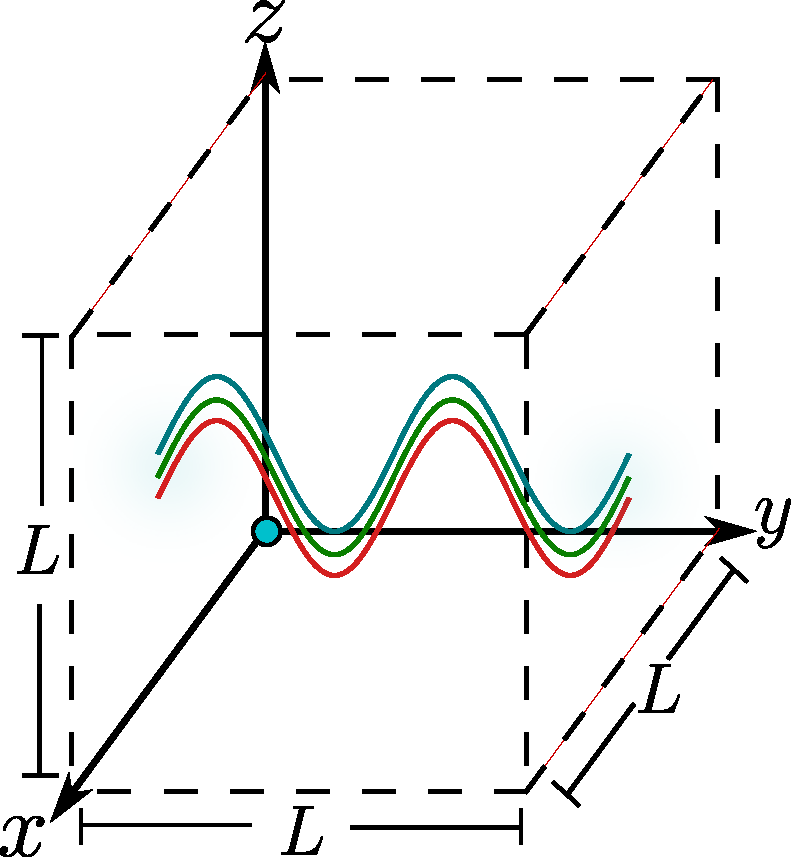
\includegraphics[width=0.45\textwidth]{Capitulo 5/Figuras/CavidadL.pdf}
        \caption{Campo eléctrico en todos sus modos confinado en una cavidad con paredes conductoras perfectas}
        \label{fig:cavidad}
    \end{figure}

   Para desarrollar la teoría cuántica del campo electromagnético, resulta conveniente trabajar con un sistema confinado en una región finita del espacio (ver figura \ref{fig:cavidad}). La cavidad resonante proporciona el escenario ideal: un recinto cerrado con paredes perfectamente conductoras que imponen condiciones de frontera bien definidas. Este modelo, aunque idealizado, captura la física esencial y permite un tratamiento matemático riguroso que luego puede generalizarse al espacio libre mediante un proceso de límite apropiado.

   Consideremos una cavidad cúbica de lado $L$, sin cargas ni corrientes en su interior. Las ecuaciones de Maxwell en el vacío toman la forma \cite{Jackson1999}
    \begin{align}
        \nabla \cdot \mathbf{E} &= 0, \\
        \nabla \cdot \mathbf{B} &= 0, \\
        \nabla \times \mathbf{E} &= -\frac{\partial \mathbf{B}}{\partial t}, \\
        \nabla \times \mathbf{B} &= \frac{1}{c^2}\frac{\partial \mathbf{E}}{\partial t},
    \end{align}
    donde $c = 1/\sqrt{\mu_0 \epsilon_0}$ es la velocidad de la luz.
    
    Para resolver estas ecuaciones, introducimos el potencial vector $\mathbf{A}(\mathbf{r}, t)$ mediante la relación $\mathbf{B} = \nabla \times \mathbf{A}$, que satisface automáticamente la condición $\nabla \cdot \mathbf{B} = 0$. La ley de Faraday implica entonces que $\nabla \times (\mathbf{E} + \partial\mathbf{A}/\partial t) = 0$, de donde podemos escribir
    \begin{equation}
        \mathbf{E} = -\nabla \Phi - \frac{\partial \mathbf{A}}{\partial t}
    \end{equation}
    para algún potencial escalar $\Phi$.
    
    Los potenciales $\mathbf{A}$ y $\Phi$ no están determinados unívocamente por los campos físicos $\mathbf{E}$ y $\mathbf{B}$; existe la libertad de gauge. Adoptamos el gauge de Coulomb, definido por la condición
    \begin{equation}
        \nabla \cdot \mathbf{A} = 0.
    \end{equation}
    
    Esta elección tiene una consecuencia importante. En ausencia de cargas, la ecuación $\nabla \cdot \mathbf{E} = 0$ junto con el gauge de Coulomb implica $\nabla^2 \Phi = 0$. En una cavidad cerrada, la única solución compatible con condiciones de frontera finitas es $\Phi = 0$. Los campos quedan entonces expresados exclusivamente en términos del potencial vector transversal:
    \begin{equation}
        \mathbf{E} = -\frac{\partial \mathbf{A}}{\partial t}, \quad \mathbf{B} = \nabla \times \mathbf{A}.
    \end{equation}
    
    Sustituyendo en la ecuación de Ampère-Maxwell y utilizando la identidad $\nabla \times (\nabla \times \mathbf{A}) = \nabla(\nabla \cdot \mathbf{A}) - \nabla^2 \mathbf{A}$, obtenemos la ecuación de onda
    \begin{equation}
        \nabla^2 \mathbf{A} - \frac{1}{c^2}\frac{\partial^2 \mathbf{A}}{\partial t^2} = 0.
    \end{equation}
    
    \section{Modos normales de la cavidad}
    
    Las paredes conductoras imponen que las componentes tangenciales del campo eléctrico se anulen en las fronteras. Buscamos soluciones mediante separación de variables, expandiendo el potencial vector en una serie de modos normales:
    \begin{equation}
        \mathbf{A}(\mathbf{r}, t) = \sum_{\mathbf{k},\lambda} q_{\mathbf{k},\lambda}(t) \, \mathbf{u}_{\mathbf{k},\lambda}(\mathbf{r}).
    \end{equation}
    
    Las funciones de modo $\mathbf{u}_{\mathbf{k},\lambda}(\mathbf{r})$ satisfacen la ecuación de Helmholtz $\nabla^2 \mathbf{u} + k^2 \mathbf{u} = 0$ junto con las condiciones de frontera. Para la cavidad cúbica, las soluciones involucran productos de funciones seno y coseno, y las condiciones de frontera cuantizan los componentes del vector de onda:
    \begin{equation}
        k_i = \frac{n_i \pi}{L}, \quad n_i = 0, 1, 2, 3, \ldots \quad (i = x, y, z).
    \end{equation}
    
    Cada vector $\mathbf{k}$ admite dos polarizaciones independientes, etiquetadas por $\lambda = 1, 2$. El gauge de Coulomb impone la condición de transversalidad $\mathbf{k} \cdot \hat{\boldsymbol{\epsilon}}_{\mathbf{k},\lambda} = 0$, de modo que los vectores de polarización son perpendiculares a la dirección de propagación. La frecuencia de cada modo está determinada por la relación de dispersión
    \begin{equation}
        \omega_{\mathbf{k}} = c\|\mathbf{k}\| = \frac{c\pi}{L}\sqrt{n_x^2 + n_y^2 + n_z^2}.
    \end{equation}
    
    Elegimos las funciones de modo normalizadas según
    \begin{equation}
        \int_V \mathbf{u}_{\mathbf{k},\lambda}(\mathbf{r}) \cdot \mathbf{u}_{\mathbf{k}',\lambda'}^*(\mathbf{r}) \, d^3r = \delta_{\mathbf{k},\mathbf{k}'}\delta_{\lambda,\lambda'},
    \end{equation}
    donde la integral se extiende sobre el volumen $V = L^3$ de la cavidad.
    
    Sustituyendo la expansión modal en la ecuación de onda y utilizando la ortogonalidad de las funciones de modo, encontramos que cada amplitud $q_{\mathbf{k},\lambda}(t)$ satisface
    \begin{equation}
        \ddot{q}_{\mathbf{k},\lambda}(t) + \omega_{\mathbf{k}}^2 q_{\mathbf{k},\lambda}(t) = 0.
    \end{equation}
    
    Esta es la ecuación de un oscilador armónico de frecuencia $\omega_{\mathbf{k}}$. Hemos llegado a un resultado fundamental: el campo electromagnético en una cavidad es dinámicamente equivalente a una colección infinita de osciladores armónicos independientes, uno por cada modo $(\mathbf{k}, \lambda)$.

    La energía total del campo electromagnético contenido en la cavidad es \cite{Jackson1999}
    \begin{equation}
        H = \frac{1}{2}\int_V \left(\epsilon_0 \|\mathbf{E}\|^2 + \frac{1}{\mu_0}\|\mathbf{B}\|^2\right) d^3r.
    \end{equation}
    
    Expresando los campos en términos del potencial vector y sustituyendo la expansión modal, el cálculo procede como sigue. Para el término eléctrico, usando $\mathbf{E} = -\partial\mathbf{A}/\partial t$:
    \begin{equation}
        \int_V \epsilon_0 \left\|\frac{\partial \mathbf{A}}{\partial t}\right\|^2 d^3r = \epsilon_0 \sum_{\mathbf{k},\lambda} |\dot{q}_{\mathbf{k},\lambda}|^2,
    \end{equation}
    donde hemos empleado la ortonormalidad de las funciones de modo.
    
    Para el término magnético, utilizamos que $\int_V \|\nabla \times \mathbf{u}_{\mathbf{k},\lambda}\|^2 d^3r = k^2 = \omega_{\mathbf{k}}^2/c^2$, lo cual conduce a
    \begin{equation}
        \int_V \frac{1}{\mu_0}\|\nabla \times \mathbf{A}\|^2 d^3r = \epsilon_0 \sum_{\mathbf{k},\lambda} \omega_{\mathbf{k}}^2 |q_{\mathbf{k},\lambda}|^2.
    \end{equation}
    
    Combinando ambas contribuciones, el Hamiltoniano total toma la forma
    \begin{equation}
        H = \frac{\epsilon_0}{2} \sum_{\mathbf{k},\lambda} \left(|\dot{q}_{\mathbf{k},\lambda}|^2 + \omega_{\mathbf{k}}^2 |q_{\mathbf{k},\lambda}|^2\right).
    \end{equation}
    
    Definiendo las variables canónicas $Q_{\mathbf{k},\lambda} = \sqrt{\epsilon_0} \, q_{\mathbf{k},\lambda}$ y $P_{\mathbf{k},\lambda} = \sqrt{\epsilon_0} \, \dot{q}_{\mathbf{k},\lambda}$, el Hamiltoniano adopta la forma estándar de una suma de osciladores armónicos:
    \begin{equation}
        H = \sum_{\mathbf{k},\lambda} \frac{1}{2}\left(P_{\mathbf{k},\lambda}^2 + \omega_{\mathbf{k}}^2 Q_{\mathbf{k},\lambda}^2\right).
    \end{equation}

    \subsection{Cuantización del campo electromagnético}

        Habiendo establecido que el campo electromagnético clásico en una cavidad es equivalente a un conjunto de osciladores armónicos, procedemos ahora a su cuantización. El procedimiento sigue el esquema canónico: promovemos las variables dinámicas a operadores y reemplazamos los corchetes de Poisson por conmutadores.

        Las variables canónicas $Q_{\mathbf{k},\lambda}$ y $P_{\mathbf{k},\lambda}$ se convierten en operadores hermitianos $\hat{Q}_{\mathbf{k},\lambda}$ y $\hat{P}_{\mathbf{k},\lambda}$ que satisfacen las relaciones de conmutación
        \begin{equation}
            [\hat{Q}_{\mathbf{k},\lambda}, \hat{P}_{\mathbf{k}',\lambda'}] = i\hbar \delta_{\mathbf{k},\mathbf{k}'}\delta_{\lambda,\lambda'},
        \end{equation}
        mientras que los conmutadores entre operadores del mismo tipo se anulan:
        \begin{equation}
            [\hat{Q}_{\mathbf{k},\lambda}, \hat{Q}_{\mathbf{k}',\lambda'}] = [\hat{P}_{\mathbf{k},\lambda}, \hat{P}_{\mathbf{k}',\lambda'}] = 0.
        \end{equation}

        Para el oscilador armónico cuántico, resulta conveniente introducir combinaciones lineales de los operadores de posición y momento que simplifican la estructura algebraica. Definimos el operador de aniquilación
        \begin{equation}
            \hat{a}_{\mathbf{k},\lambda} = \sqrt{\frac{\omega_{\mathbf{k}}}{2\hbar}}\hat{Q}_{\mathbf{k},\lambda} + \frac{i}{\sqrt{2\hbar\omega_{\mathbf{k}}}}\hat{P}_{\mathbf{k},\lambda}
        \end{equation}
        y el operador de creación como su adjunto hermitiano
        \begin{equation}
            \hat{a}^\dagger_{\mathbf{k},\lambda} = \sqrt{\frac{\omega_{\mathbf{k}}}{2\hbar}}\hat{Q}_{\mathbf{k},\lambda} - \frac{i}{\sqrt{2\hbar\omega_{\mathbf{k}}}}\hat{P}_{\mathbf{k},\lambda}.
        \end{equation}
        
        Para determinar el álgebra de estos operadores, calculamos su conmutador. Usando las relaciones de conmutación canónicas:
        \begin{align}
            [\hat{a}_{\mathbf{k},\lambda}, \hat{a}^\dagger_{\mathbf{k}',\lambda'}] &= \frac{\omega_{\mathbf{k}}}{2\hbar}[\hat{Q}_{\mathbf{k},\lambda}, \hat{Q}_{\mathbf{k}',\lambda'}] - \frac{i}{2\hbar}\sqrt{\frac{\omega_{\mathbf{k}}}{\omega_{\mathbf{k}'}}}[\hat{Q}_{\mathbf{k},\lambda}, \hat{P}_{\mathbf{k}',\lambda'}] \nonumber \\
            &\quad + \frac{i}{2\hbar}\sqrt{\frac{\omega_{\mathbf{k}'}}{\omega_{\mathbf{k}}}}[\hat{P}_{\mathbf{k},\lambda}, \hat{Q}_{\mathbf{k}',\lambda'}] + \frac{1}{2\hbar\sqrt{\omega_{\mathbf{k}}\omega_{\mathbf{k}'}}}[\hat{P}_{\mathbf{k},\lambda}, \hat{P}_{\mathbf{k}',\lambda'}].
        \end{align}
        
        Los conmutadores $[\hat{Q}, \hat{Q}]$ y $[\hat{P}, \hat{P}]$ se anulan. Utilizando $[\hat{Q}_{\mathbf{k},\lambda}, \hat{P}_{\mathbf{k}',\lambda'}] = i\hbar\delta_{\mathbf{k},\mathbf{k}'}\delta_{\lambda,\lambda'}$ y $[\hat{P}_{\mathbf{k},\lambda}, \hat{Q}_{\mathbf{k}',\lambda'}] = -i\hbar\delta_{\mathbf{k},\mathbf{k}'}\delta_{\lambda,\lambda'}$, obtenemos
        \begin{equation}
            [\hat{a}_{\mathbf{k},\lambda}, \hat{a}^\dagger_{\mathbf{k}',\lambda'}] = \frac{1}{2}\delta_{\mathbf{k},\mathbf{k}'}\delta_{\lambda,\lambda'} + \frac{1}{2}\delta_{\mathbf{k},\mathbf{k}'}\delta_{\lambda,\lambda'} = \delta_{\mathbf{k},\mathbf{k}'}\delta_{\lambda,\lambda'}.
        \end{equation}
        
        Por construcción, también se tiene $[\hat{a}_{\mathbf{k},\lambda}, \hat{a}_{\mathbf{k}',\lambda'}] = [\hat{a}^\dagger_{\mathbf{k},\lambda}, \hat{a}^\dagger_{\mathbf{k}',\lambda'}] = 0$. Estas son las relaciones de conmutación bosónicas características de los fotones.
        
        Las relaciones pueden invertirse para expresar los operadores de posición y momento en términos de los operadores de escalera:
        \begin{align}
            \hat{Q}_{\mathbf{k},\lambda} &= \sqrt{\frac{\hbar}{2\omega_{\mathbf{k}}}}\left(\hat{a}_{\mathbf{k},\lambda} + \hat{a}^\dagger_{\mathbf{k},\lambda}\right), \\
            \hat{P}_{\mathbf{k},\lambda} &= i\sqrt{\frac{\hbar\omega_{\mathbf{k}}}{2}}\left(\hat{a}^\dagger_{\mathbf{k},\lambda} - \hat{a}_{\mathbf{k},\lambda}\right).
        \end{align}
 
        Estas relaciones expresan que modos diferentes son dinámicamente independientes; cada par $(\mathbf{k}, \lambda)$ constituye un grado de libertad cuántico separado.

        Los campos electromagnéticos se promueven a operadores sustituyendo las amplitudes clásicas por operadores cuánticos. El operador de campo eléctrico resulta

        \begin{equation}
            \hat{E}(\mathbf{r}, t) = i\sum_{\mathbf{k},\lambda} \sqrt{\frac{\hbar\omega_{\mathbf{k}}}{2\epsilon_0 V}} \left(\hat{a}_{\mathbf{k},\lambda} e^{-i\omega_{\mathbf{k}} t} - \hat{a}^\dagger_{\mathbf{k},\lambda} e^{i\omega_{\mathbf{k}} t}\right) \hat{\boldsymbol{\epsilon}}_{\mathbf{k},\lambda} f_{\mathbf{k}}(\mathbf{r}),
        \end{equation}
        donde $f_{\mathbf{k}}(\mathbf{r})$ representa la dependencia espacial del modo y $V = L^3$ es el volumen de la cavidad.
        
        Análogamente, el operador de campo magnético es
        \begin{equation}
            \hat{B}(\mathbf{r}, t) = i\sum_{\mathbf{k},\lambda} \sqrt{\frac{\hbar}{2\epsilon_0\omega_{\mathbf{k}} V}} \left(\hat{a}_{\mathbf{k},\lambda} e^{-i\omega_{\mathbf{k}} t} - \hat{a}^\dagger_{\mathbf{k},\lambda} e^{i\omega_{\mathbf{k}} t}\right) (\mathbf{k} \times \hat{\boldsymbol{\epsilon}}_{\mathbf{k},\lambda}) g_{\mathbf{k}}(\mathbf{r}).
        \end{equation}
        
        Ambos operadores son hermitianos, como corresponde a observables físicos. La combinación particular de operadores de creación y aniquilación, con sus respectivas fases temporales, garantiza que $\hat{E}^\dagger = \hat{E}$ y $\hat{B}^\dagger = \hat{B}$.


    \subsection{El Oscilador Armónico Cuántico de la radiación y los Estados de Fock}
        
        La estructura matemática que hemos desarrollado conduce naturalmente al oscilador armónico cuántico, uno de los sistemas más importantes de toda la física teórica. En el contexto de la óptica cuántica, las excitaciones del oscilador armónico corresponden a los fotones.

        Partimos del Hamiltoniano de un modo individual, $\hat{H}_{\mathbf{k},\lambda} = \frac{1}{2}(\hat{P}^2 + \omega^2\hat{Q}^2)$, donde omitimos los subíndices para simplificar la notación. Sustituyendo las expresiones de $\hat{Q}$ y $\hat{P}$ en términos de $\hat{a}$ y $\hat{a}^\dagger$:
        \begin{equation}
            \hat{H} = \frac{1}{2}\left[-\frac{\hbar\omega}{2}(\hat{a}^\dagger - \hat{a})^2 + \omega^2 \cdot \frac{\hbar}{2\omega}(\hat{a} + \hat{a}^\dagger)^2\right].
        \end{equation}
        
        Expandiendo los cuadrados y simplificando:
        \begin{align}
            (\hat{a}^\dagger - \hat{a})^2 &= \hat{a}^\dagger\hat{a}^\dagger - \hat{a}^\dagger\hat{a} - \hat{a}\hat{a}^\dagger + \hat{a}\hat{a}, \\
            (\hat{a} + \hat{a}^\dagger)^2 &= \hat{a}\hat{a} + \hat{a}\hat{a}^\dagger + \hat{a}^\dagger\hat{a} + \hat{a}^\dagger\hat{a}^\dagger.
        \end{align}
        
        Al restar estas expresiones, los términos $\hat{a}^\dagger\hat{a}^\dagger$ y $\hat{a}\hat{a}$ se cancelan, quedando
        \begin{equation}
            (\hat{a} + \hat{a}^\dagger)^2 - (\hat{a}^\dagger - \hat{a})^2 = 2(\hat{a}\hat{a}^\dagger + \hat{a}^\dagger\hat{a}).
        \end{equation}
        
        Usando la relación de conmutación $[\hat{a}, \hat{a}^\dagger] = 1$, podemos escribir $\hat{a}\hat{a}^\dagger = \hat{a}^\dagger\hat{a} + 1$, de donde $\hat{a}\hat{a}^\dagger + \hat{a}^\dagger\hat{a} = 2\hat{a}^\dagger\hat{a} + 1$. El Hamiltoniano resulta
        \begin{equation}
            \hat{H} = \hbar\omega\left(\hat{a}^\dagger\hat{a} + \frac{1}{2}\right).
        \end{equation}
        
    \section{El operador número}
        
        Definimos el operador número como
        \begin{equation}
            \hat{N} \equiv \hat{a}^\dagger\hat{a}.
        \end{equation}
        
        Este operador cuenta el número de excitaciones (fotones) en el modo. En términos del operador número, el Hamiltoniano de cada modo se escribe
        \begin{equation}
            \hat{H}_{\mathbf{k},\lambda} = \hbar\omega_{\mathbf{k}}\left(\hat{N}_{\mathbf{k},\lambda} + \frac{1}{2}\right),
        \end{equation}
        y el Hamiltoniano total del campo electromagnético es la suma sobre todos los modos:
        \begin{equation}
            \hat{H} = \sum_{\mathbf{k},\lambda} \hbar\omega_{\mathbf{k}}\left(\hat{N}_{\mathbf{k},\lambda} + \frac{1}{2}\right).
        \end{equation}
        
        Para entender la acción de los operadores de escalera, calculamos sus conmutadores con el operador número. Usando la identidad $[AB, C] = A[B, C] + [A, C]B$:
        \begin{align}
            [\hat{N}, \hat{a}] &= [\hat{a}^\dagger\hat{a}, \hat{a}] = \hat{a}^\dagger[\hat{a}, \hat{a}] + [\hat{a}^\dagger, \hat{a}]\hat{a} = 0 - \hat{a} = -\hat{a}, \\
            [\hat{N}, \hat{a}^\dagger] &= [\hat{a}^\dagger\hat{a}, \hat{a}^\dagger] = \hat{a}^\dagger[\hat{a}, \hat{a}^\dagger] + [\hat{a}^\dagger, \hat{a}^\dagger]\hat{a} = \hat{a}^\dagger \cdot 1 + 0 = \hat{a}^\dagger.
        \end{align}
        
        Estas relaciones tienen una interpretación inmediata. Si $\ket{n}$ es un autoestado del operador número con autovalor $n$, entonces
        \begin{equation}
            \hat{N}(\hat{a}\ket{n}) = \hat{a}(\hat{N} - 1)\ket{n} = (n-1)(\hat{a}\ket{n}),
        \end{equation}
        lo que muestra que $\hat{a}\ket{n}$ es autoestado con autovalor $n-1$. Análogamente, $\hat{a}^\dagger\ket{n}$ es autoestado con autovalor $n+1$. Por esto $\hat{a}$ se llama operador de aniquilación (reduce el número de excitaciones en uno) y $\hat{a}^\dagger$ se llama operador de creación (aumenta el número en uno).

        Para determinar los autovalores permitidos del operador número, observamos primero que $\hat{N}$ es semidefinido positivo:
        \begin{equation}
            \bra{\psi}\hat{N}\ket{\psi} = \bra{\psi}\hat{a}^\dagger\hat{a}\ket{\psi} = \|\hat{a}\ket{\psi}\|^2 \geq 0.
        \end{equation}
        
        Por tanto, todos los autovalores son no negativos. Si existiera un autovalor no entero $n = m + \epsilon$ con $0 < \epsilon < 1$ y $m$ entero, la aplicación sucesiva del operador de aniquilación produciría eventualmente un autovalor negativo, lo cual es imposible. Concluimos que los autovalores deben ser enteros no negativos: $n = 0, 1, 2, 3, \ldots$
        
        El estado con $n = 0$ es el estado de vacío $\ket{0}$, caracterizado por
        \begin{equation}
            \hat{a}\ket{0} = 0.
        \end{equation}
        
        Los estados con $n$ fotones, llamados estados de Fock o estados número, se construyen aplicando el operador de creación repetidamente:
        \begin{equation}
            \ket{n} = \frac{(\hat{a}^\dagger)^n}{\sqrt{n!}}\ket{0}.
        \end{equation}
        
        El factor $1/\sqrt{n!}$ asegura la normalización $\braket{n|n} = 1$. Las acciones de los operadores de escalera sobre estos estados son
        \begin{align}
            \hat{a}\ket{n} &= \sqrt{n}\ket{n-1}, \\
            \hat{a}^\dagger\ket{n} &= \sqrt{n+1}\ket{n+1}.
        \end{align}
        
        La energía del estado con $n$ fotones en el modo $(\mathbf{k}, \lambda)$ es
        \begin{equation}
            E_n = \hbar\omega_{\mathbf{k}}\left(n + \frac{1}{2}\right).
        \end{equation}
        
        Los niveles de energía están igualmente espaciados, con separación $\hbar\omega_{\mathbf{k}}$ entre niveles consecutivos. Esta es precisamente la energía de un fotón de frecuencia $\omega_{\mathbf{k}}$, confirmando la interpretación corpuscular: cada excitación del campo corresponde a un fotón.

    \subsection{La energía del vacío cuántico}
        
        El término $\frac{1}{2}\hbar\omega_{\mathbf{k}}$ representa la energía de punto cero del modo, presente incluso cuando no hay fotones. La energía total del vacío electromagnético es
        \begin{equation}
            E_{\text{vacío}} = \frac{1}{2}\sum_{\mathbf{k},\lambda} \hbar\omega_{\mathbf{k}}.
        \end{equation}
        
        Esta suma diverge, pues hay infinitos modos. En la práctica, esta contribución infinita se elimina mediante técnicas de renormalización o redefiniendo el Hamiltoniano con ordenamiento normal, donde todos los operadores de creación se colocan a la izquierda de los de aniquilación.
        
        Sin embargo, la energía del vacío tiene consecuencias físicas observables. El efecto Casimir \cite{Casimir1948}, la fuerza atractiva entre dos placas conductoras paralelas en el vacío, es una manifestación directa de las fluctuaciones cuánticas del campo electromagnético.

    \subsection{Fluctuaciones del vacío}

        Dado que ya hemos descrito al campo eléctrico como una entidad que oscila de forma cuantizada de la misma manera que un oscilador armónico, podemos estudiar algunas de sus propiedades en el espacio número o de Fock. Para un modo estacionario único, el operador de campo eléctrico se escribe
        \begin{equation}\label{eq:CampoModoUnico}
            \hat{E}_{x}(z) = \mathcal{E}_{0}\sin(kz)\left(\hat{a} + \hat{a}^{\dagger}\right),
            \qquad
            \mathcal{E}_{0} = \sqrt{\frac{\hbar\omega}{\epsilon_{0}V}},
        \end{equation}
        donde $\mathcal{E}_{0}$ es la amplitud del campo asociada a un solo cuanto y no debe confundirse con la permitividad $\epsilon_{0}$ del vacío. Su valor esperado en un estado número se anula,
        \begin{equation}
            \left\langle \hat{E}_{x} \right\rangle_{n} = \mathcal{E}_{0}\sin(kz)\left[\bra{n}\hat{a}\ket{n} + \bra{n}\hat{a}^{\dagger}\ket{n}\right] = 0,
        \end{equation}
        porque $\hat{a}$ y $\hat{a}^{\dagger}$ conectan estados con números de fotones distintos y sus elementos diagonales son nulos. \textbf{Un estado con un número definido de fotones no tiene campo eléctrico medio}, resultado que a primera vista desconcierta y que expresa el hecho de que un estado número no posee fase definida, como se discutirá en detalle más adelante.

        Este resultado motiva a pensar en una incertidumbre intrínseca entre el número de fotones $n$ y el valor del campo, lo cual se evidencia calculando su conmutador,
        \begin{equation}
            \left[\hat{N}, \hat{E}_{x}\right] = \mathcal{E}_{0}\sin(kz)\left(\hat{a}^{\dagger} -\hat{a}\right)
            \quad\Longrightarrow\quad
            \Delta \hat{N}\,\Delta\hat{E}_{x} \geq \frac{1}{2}\mathcal{E}_{0}\left|\sin(kz)\right|\left|\left\langle\hat{a}^{\dagger} - \hat{a}\right\rangle\right|,
        \end{equation}
        donde la desigualdad es la relación de Robertson aplicada a este par de observables.

        El valor cuadrático medio, en cambio, no se anula,
        \begin{equation}
            \left\langle \hat{E}^{2}_{x}\right\rangle_{n} = \mathcal{E}_{0}^{2}\sin^{2}(kz)\,\bra{n}\left(\hat{a}^{\dagger}\right)^{2} + \hat{a}^{2} + \hat{a}^{\dagger}\hat{a} + \hat{a}\hat{a}^{\dagger}\ket{n} = 2\,\mathcal{E}_{0}^{2}\sin^{2}(kz)\left(n+ \frac{1}{2}\right),
        \end{equation}
        puesto que los dos primeros términos tienen valor esperado nulo y los dos últimos aportan $n$ y $n+1$ respectivamente. La incertidumbre del campo es entonces
        \begin{equation}
            \Delta \hat{E}_{x} = \sqrt{\left\langle \hat{E}^{2}_{x}\right\rangle - \left\langle \hat{E}_{x}\right\rangle^{2}} = \sqrt{2}\,\mathcal{E}_{0}\left|\sin(kz)\right|\sqrt{n+\frac{1}{2}} .
        \end{equation}

        Si nos fijamos en el estado de vacío $n = 0$, la incertidumbre del campo no se anula sino que vale $\mathcal{E}_{0}|\sin(kz)|/\sqrt{2}$, y este resultado es el que se conoce como la fluctuación del vacío cuántico del campo electromagnético. Es un pilar fundamental para el desarrollo de la electrodinámica cuántica, puesto que permite dar una explicación precisa y compatible con los resultados experimentales de diferentes fenómenos como lo son el corrimiento de Lamb, el efecto Casimir o la emisión espontánea de fotones \citep{Introd-QO}.
%Hablar 

\section{Los estados coherentes}

    Vamos a encontrar una familia de estados realmente importantes, primero encontrando cierta familia de estados especiales que a su vez son los autovalores del operador de aniquilación $\hat{a}$, sabemos que la mecánica cuántica debe producir los mismos resultados que la mecánica clásica en el caso límite en el que el oscilador armónico tiene una energía mucho mayor que la del cuanto de energía $\hbar \omega$.

    Por lo tanto, podemos plantear la siguiente pregunta: ¿es posible construir estados mecánicos cuánticos que conduzcan a predicciones físicas casi idénticas a las clásicas, al menos para un oscilador macroscópico? Veremos en este complemento que existen tales estados cuánticos: son superposiciones lineales coherentes de todos los estados. Los llamaremos \textit{estados cuasi-clásicos} o \textit{estados coherentes del oscilador armónico.}

    El problema que estamos considerando aquí es de gran interés general en la mecánica cuántica. Como bien se sabe en la mecánica cuántica muchos sistemas físicos pueden ser comparados con un oscilador armónico, al menos en una primera aproximación \cite{cohen1986quantum}. Para todos estos sistemas, es importante entender, en el marco de la mecánica cuántica, cómo pasar gradualmente del caso en el que los resultados dados por la aproximación clásica son suficientes al caso en el que los efectos cuánticos son preponderantes.

    La radiación electromagnética es un ejemplo muy importante de tal sistema. Dependiendo del experimento, revela su naturaleza mecánico cuántica o bien puede ser tratada clásicamente. Los estados coherentes de la radiación electromagnética fueron introducidos por Glauber y se utilizan actualmente en el campo de la óptica cuántica.\\

    Definimos los estados coherentes $\ket{\alpha}$ como los autoestados o estados propios del operador de aniquilación $\hat{a}$

    \begin{equation}
        \hat{a}\ket{\alpha} = \alpha\ket{\alpha}\;,
    \end{equation}

    podemos encontrar de muchas formas estos estados coherentes pero como conocemos bien los estados número $\ket{n}$ podemos encontrar los estados $\ket{\alpha}$ como una combinación lineal de los estados números pues estos conforman una base completa y ortonormal, en este orden de ideas tenemos

    \begin{equation}
        \ket{\alpha} = \sum_m C_m \ket{m}\;,
    \end{equation}

    \begin{equation}
        \hat{a}\ket{\alpha} = \sum_m C_m \sqrt{m}\ket{m-1} = \alpha \sum_n C_n \ket{n}\;,
    \end{equation}

    para el lado izquierdo de la ecuación vemos que se iguala al lado derecho cuando $m = n +1$ entonces tenemos la siguiente ecuación para los coeficientes de la expansión 
    
    \begin{equation}\label{eq:coefcnmahuno}
        C_{n+1}\sqrt{n + 1} = \alpha C_n \rightarrow C_{n+1} = \frac{\alpha}{\sqrt{n + 1}}C_n \;.
    \end{equation}

    La relación de recurrencia \ref{eq:coefcnmahuno} muestra un patrón en los coeficientes de la expansión, si evaluamos los primeros tres términos podemos ver dicho patrón:

    \begin{align*}
        C_1 = \frac{\alpha}{\sqrt{1}}C_0\;,\\
        C_2 = \frac{\alpha}{\sqrt{2}}C_1 = \frac{\alpha^2}{\sqrt{2\cdot 1}}C_0\;,\\
        C_3 = \frac{\alpha}{\sqrt{3}}C_2 = \frac{\alpha^3}{\sqrt{3\cdot 2\cdot 1}}C_0\;.
    \end{align*}

    Es fácil ver que el enésimo coeficiente se puede expresar en términos del primer coeficiente de la siguiente manera,

    \begin{equation}
        C_n = \frac{\alpha^n}{\sqrt{n!}}C_0\;.
    \end{equation}

    Vemos que cuando $C_0$ está fijo, es decir, es constante, el enésimo coeficiente también lo será esto implica que el estado $\ket{\alpha}$ es único o a lo mucho varía en una constante de proporcionalidad, para determinar el coeficiente $C_0$ vamos a aprovecharnos de que el estado $\ket{\alpha}$ debe estar normalizado, entonces tenemos la siguiente ecuación 

    \begin{equation}
        \sum_n |C_n|^2 = 1\;,
    \end{equation}

    \begin{equation}
        \sum_n \frac{|\alpha|^{2n}}{n!}|C_0|^2 = 1\;,
    \end{equation}

    pero podemos darnos cuenta que la suma no es más que una expansión en series de Taylor de un exponencial,

    \begin{equation}
        |C_0|^2 e^{|\alpha|^2} = 1 \rightarrow C_0 = e^{-|\alpha|^2/2}\;.
    \end{equation}

    Ahora, podemos determinar los estados coherentes como:

    \begin{equation}\label{eq:CoherentStates}
        \ket{\alpha} = e^{-|\alpha|^2/2}\sum_n \frac{\alpha^n}{\sqrt{n!}}\ket{n}\;.
    \end{equation}

    Vamos ahora a considerar el valor esperado del operador de campo eléctrico esto con el objetivo de hacer la comparación con los valores esperados de la mecánica clásica,

    \begin{equation}
        \hat{E}_x(\Vec{r},t) = i\left(\frac{\hbar \omega}{2\epsilon_0V}\right)^{1/2}\left[\hat{a}e^{i(\Vec{k}\cdot \Vec{r} - \omega t)} - \hat{a}^{\dagger}e^{-i(\Vec{k}\cdot\Vec{r} - \omega t)} \right]\;.
    \end{equation}

    Obtenemos entonces:

    \begin{equation}\label{eq:espEx}
        \bra{\alpha} \hat{E}_x \ket{\alpha} = i\left(\frac{\hbar \omega}{2\epsilon_0V}\right)^{1/2}\left[\alpha e^{i(\Vec{k}\cdot \Vec{r} - \omega t)} - \alpha^{*}e^{-i(\Vec{k}\cdot\Vec{r} - \omega t)} \right]\;.
    \end{equation}

    Ahora, como $\alpha$ puede ser, en general, un número complejo o real, lo podemos escribir en forma polar ($\alpha = |\alpha|e^{i\theta}$) e introducirlo a la ecuación \ref{eq:espEx}

    \begin{equation}
        \bra{\alpha} \hat{E}_x \ket{\alpha} = 2|\alpha|\left(\frac{\hbar \omega}{2\epsilon_0V}\right)^{1/2}\sin(\omega t - \Vec{k}\cdot \Vec{r} - \theta).
    \end{equation}

    ¿Esto tiene sentido? Si resolvemos la ecuación de onda del campo electromagnético con las condiciones de frontera de la cavidad, vemos que tanto el valor esperado cuántico en la base de los estados coherentes como los modos de oscilación de la radiación en una cavidad son semejantes.\\

    De la misma forma podemos calcular el valor esperado cuadrático del campo eléctrico, el cual da

    \begin{equation}
        \bra{\alpha}\hat{E}_x^2\ket{\alpha} = \frac{\hbar\omega}{2\epsilon_0 V}\left[1 + 4|\alpha|^2\sin^2(\omega t - \Vec{k}\cdot \Vec{r} - \theta) \right]\;.
    \end{equation}

    De esta forma podemos calcular la incertidumbre del campo eléctrico, teniendo en cuenta que está dada por $\Delta E_x = \sqrt{\langle \hat{E}_x^{2}\rangle - \langle \hat{E}_x\rangle^{2}}$, 

    \begin{equation}
        \Delta E_x = \left[\frac{\hbar\omega}{2\epsilon_0 V}\left[1 + 4|\alpha|^2\sin^2(\omega t - \Vec{k}\cdot \Vec{r} - \theta) \right] - 4|\alpha|^2\left(\frac{\hbar \omega}{2\epsilon_0V}\right)\sin^2(\omega t - \Vec{k}\cdot \Vec{r} - \theta) \right]^{1/2}\;,
    \end{equation}

    \begin{equation}
        \Delta E_x = \left(\frac{\hbar \omega}{2\epsilon_0 V} \right)^{1/2}\;,
    \end{equation}

    es la misma incertidumbre que para el del estado de vacío. Vemos que los estados coherentes tienen bien ganado su nombre de estados cuasi-clásicos pues el valor esperado del campo eléctrico coincide con su versión clásica pero sus fluctuaciones coinciden con las del vacío cuántico , es más si utilizamos los operadores de cuadratura tenemos la siguiente expresión:

    \begin{equation}
        \langle \left(\Delta\hat{X}_1\right)^2 \rangle_{\alpha} = \frac{1}{4} =  \langle \left(\Delta\hat{X}_2\right)^2 \rangle_{\alpha}.
    \end{equation}

    Por lo tanto, con respecto a los operadores de cuadratura de campo, los estados coherentes minimizan (de hecho, igualan) el producto de incertidumbre y muestran incertidumbres iguales, las del vacío, en cada cuadratura. De hecho, esta propiedad se puede utilizar como una definición alternativa para los estados coherentes. Considera tres operadores hermíticos, $\hat{A} , \hat{B} , \hat{C}$  que satisfacen la siguiente regla de conmutación

    \begin{equation}\label{eq:condiABC}
        \left[\hat{A} , \hat{B}\right] = i \hat{C}\;,
    \end{equation}

    del álgebra de operadores \cite{zettili2009quantum} se sabe bien que la relación de incertidumbre para dos observables cualesquiera $\hat{A}$ y $\hat{B}$ está dada por

    \begin{equation}
        \langle (\Delta\hat{A})^2 \rangle \langle (\Delta\hat{B})^2 \rangle \geq \frac{1}{4} \left|\langle [\hat{A},\hat{B}]\rangle \right|^{2}\;,
    \end{equation}

    utilizando la condición de conmutación \ref{eq:condiABC} se tiene entonces

    \begin{equation}
        \langle (\Delta\hat{A})^2 \rangle \langle (\Delta\hat{B})^2 \rangle \geq \frac{1}{4}\left|\langle \hat{C}\rangle\right|^{2}
    \end{equation}

    Los estados de mínima incertidumbre serán aquellos que convierten cumplen la igualdad, estos estados deben satisfacer la siguiente ecuación de autovalores \cite{merzbacher1998quantum}

    \begin{equation}
        \left[\hat{A} + \frac{i \langle \hat{C} \rangle}{2\langle (\triangle \hat{B})^2 \rangle} \hat{B} \right] \ket{\Psi} = \left[\langle \hat{A} \rangle + \frac{i \langle \hat{C} \rangle}{2\langle (\Delta \hat{B})^2 \rangle} \langle \hat{B} \rangle \right]\ket{\Psi}.
    \end{equation}


    Si utilizamos la relación de conmutación entre los operadores de cuadratura la ecuación de autovalores se convierte en la siguiente

    \begin{equation}
        \left[\hat{X}_1 + i\hat{X}_2 \right]\ket{\Psi} = \left[\langle \hat{X}_1 \rangle + i \langle \hat{X}_2 \rangle \right]\ket{\Psi}\;,
    \end{equation}

    donde surge \cite{gerry2005introductory} que el parámetro $\alpha$ está dado por $\alpha = \langle \hat{X}_1 \rangle + i \langle \hat{X}_2 \rangle $. Esta forma para el autovalor de los estados coherentes es bastante particular, pues por la forma que tiene podemos, a priori, especular que tenga algo que ver con el campo de Riemann-Silberstein pero la relación con dicho campo será tratada más adelante.
    
    ¿Qué interpretación física tiene $|\alpha|$? Con todo lo desarrollado hasta el momento, todo indica a que este está relacionado con la amplitud del campo (y por la forma que acabamos de encontrar para $\alpha$ lo podemos representar como un vector en el espacio de cuadratura complejo). Para ver esto, calculemos el valor esperado del número de cuantos de energía respecto a la base de estados coherentes

    \begin{equation}\label{eq:AlphaQuadrado}
        \langle n \rangle_{\alpha} = \bra{\alpha} \hat{n} \ket{\alpha} = \bra{\alpha} \hat{a}^{\dagger} \hat{a} \ket{\alpha} =\bra{\alpha} \alpha^* \alpha \ket{\alpha} = |\alpha|^2\;.
    \end{equation}

    Se puede ver entonces que $|\alpha|^2$ representa el valor esperado de cuantos de energía de la radiación, de esta misma forma podemos calcular las fluctuaciones del número de cuantos de la siguiente forma:

    \begin{equation}
        \bra{\alpha}\hat{n}^2\ket{\alpha} = \bra{\alpha}\hat{a}^{\dagger}\hat{a}\hat{a}^{\dagger}\hat{a}\ket{\alpha} = |\alpha|^4 + |\alpha|^2\;,
    \end{equation}

    \begin{equation}\label{eq:deltaEnexd}
        \Delta n = \sqrt{\langle \hat{n}^2 \rangle - \langle \hat{n} \rangle ^2} = |\alpha|\;.
    \end{equation}
    

    En este momento cabe preguntarse ¿qué está oscilando armónicamente? Si en el mundo macroscópico tenemos péndulos a pequeños ángulos o canicas oscilan en un pozo parabólico, en el contexto de la radiación ¿es el fotón el que está oscilando así? Para tratar de dar una solución a esto, primero desarrollemos la ecuación \ref{eq:CoherentStates} un poco más matemáticamente y luego veamos una representación gráfica tanto de los estados número como de los estados coherentes.\\

    Vamos a utilizar el teorema de desenlace \cite{sakurai1995modern}.

    \begin{myteo}\label{teo:Desenlace}
        Sean $\hat{A}$ y $\hat{B}$ dos operadores, que no necesariamente conmutan, se cumple que la regla de exponenciación de la suma de $\hat{A}$ y $\hat{B}$ es:

        \begin{equation}
            e^{\hat{A} + \hat{B}} = e^{\hat{A}}e^{\hat{B}}e^{-\frac{1}{2}[\hat{A},\hat{B}]} = e^{\hat{B}}e^{\hat{A}}e^{\frac{1}{2}[\hat{A},\hat{B}]}.
        \end{equation}

    \end{myteo}

    Vamos a definir el operador de desplazamiento $\hat{\mathcal{D}}$ el cual jugará un rol importante en la interpretación física de los estados coherentes. El operador de desplazamiento es

    \begin{equation}
        \hat{\mathcal{D}}(\alpha) = e^{\alpha\hat{a}^{\dagger} - \alpha^*\hat{a}},
    \end{equation}

    y utilizando el teorema \ref{teo:Desenlace} entonces queda:

    \begin{equation}
        \hat{\mathcal{D}} = e^{-\frac{1}{2}|\alpha|^2}e^{\alpha \hat{a}^{\dagger}}e^{-\alpha^*\hat{a}}.
    \end{equation}

    Podemos expandir cada uno de los exponenciales, exceptuando el primero, en series de Taylor y haremos que actúe sobre el estado de vacío $\ket{0}$.

    \begin{equation}
        e^{-\alpha^*\hat{a}} \ket{0} = \sum_{k=0}^{\infty}\frac{(-\alpha^*\hat{a})^k}{k!}\ket{0} = \ket{0}\;,
    \end{equation}

    \begin{equation}
        e^{\alpha\hat{a}^{\dagger}}\ket{0} = \sum_{n=0}^{\infty}\frac{\alpha^n}{n!}(\hat{a}^{\dagger})^n\ket{0} = \sum_{n=0}^{\infty}\frac{\alpha^n}{\sqrt{n!}}\ket{n}\;,
    \end{equation}

    En este orden de ideas, es fácil ver que aplicar el operador de desplazamiento sobre el estado de vacío $\ket{0}$ nos da origen a los estados coherentes $\ket{\alpha}$

    \begin{equation}
        \ket{\alpha} = \hat{\mathcal{D}}\ket{0}.
    \end{equation}

    Es decir, que los estados coherentes surgen al realizar desplazamientos de los estados de vacío, es decir, estados Gaussianos, los cuales oscilan como un oscilador armónico (esto se discutirá más a fondo en la siguiente subsección) ¿pero qué está oscilando? Comparemos un poco el comportamiento de estos estados respecto a los estados número ilustrados en la figura \ref{fig:EstadosNumero}.

    \begin{figure}[htbp]
        \centering
        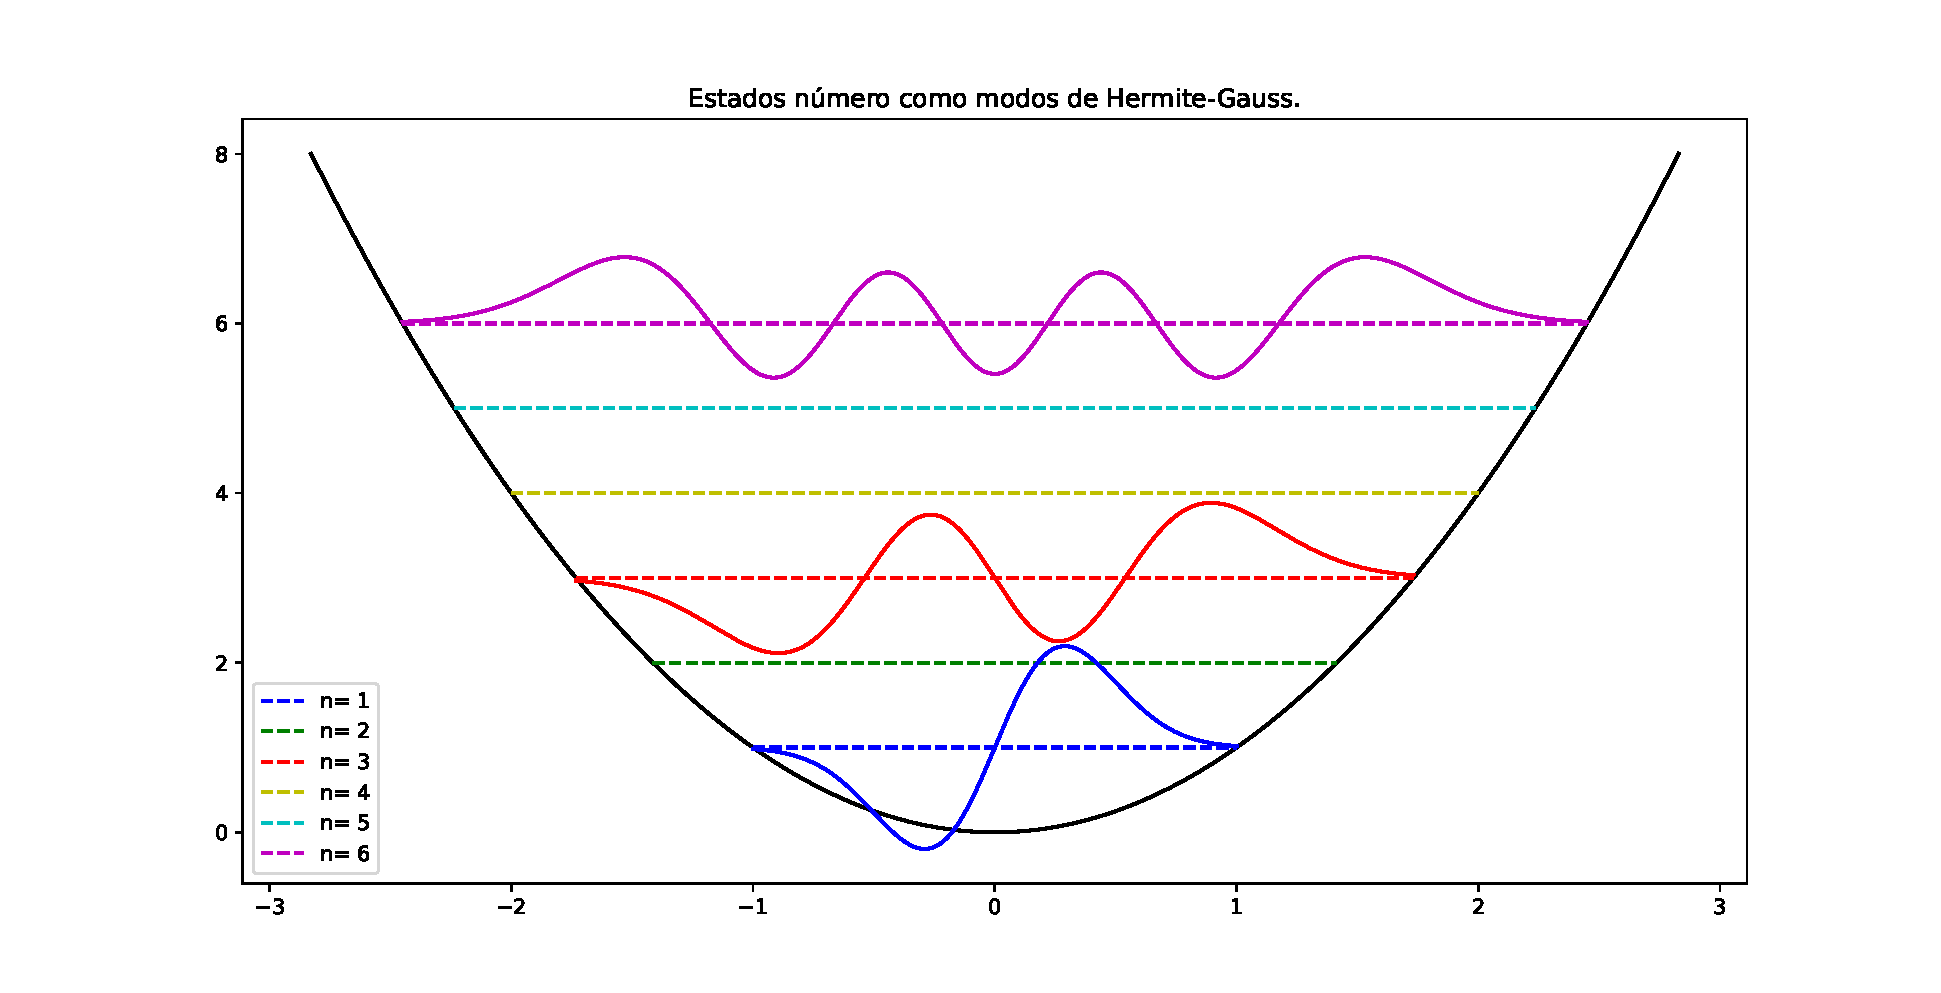
\includegraphics[width = \textwidth]{Capitulo 5/Figuras/EstadosNumero.pdf}
        \caption{Se representan gráficamente los primeros 6 niveles de energía para un oscilador harmónico cuántico, en este caso correspondiente al hamiltoniano del campo electromagnético. Para los niveles de energía; $1,3,6$ se ilustran estos estados en la base de posición, los cuales corresponden a las funciones de Hermite-Gauss.}
        \label{fig:EstadosNumero}
    \end{figure}

    Mientras que los estados número son estados estacionarios a lo largo de sus niveles de energía los estados coherentes evolucionan, en el sentido de que es un estado de vacío el cual está oscilando como un oscilador clásico pero como hemos visto, hay una relación de incertidumbre entre los operadores de campo eléctrico y magnético, no solo entre esos, sino entre los operadores de cuadratura, así que no es el fotón el que está oscilando armónicamente.\\

    Si nos remontamos a los orígenes de la mecánica cuántica, Albert Einstein hizo una gran contribución con su artículo \textit{la cuantización de la radiación} \cite{einstein20167} en la cual, en orden de que se cumpla la física cuántica de la radiación la energía de esta, de los fotones debe estar bien dirigida entonces podemos entender a los estados coherentes $\ket{\alpha}$ como los estados que me representan a nivel clásico las oscilaciones armónicas de la energía bien dirigida, estas oscilaciones se representan en la figura \ref{fig:EvolEstadosCoherentes}.

    \begin{figure}[htbp]
        \centering
        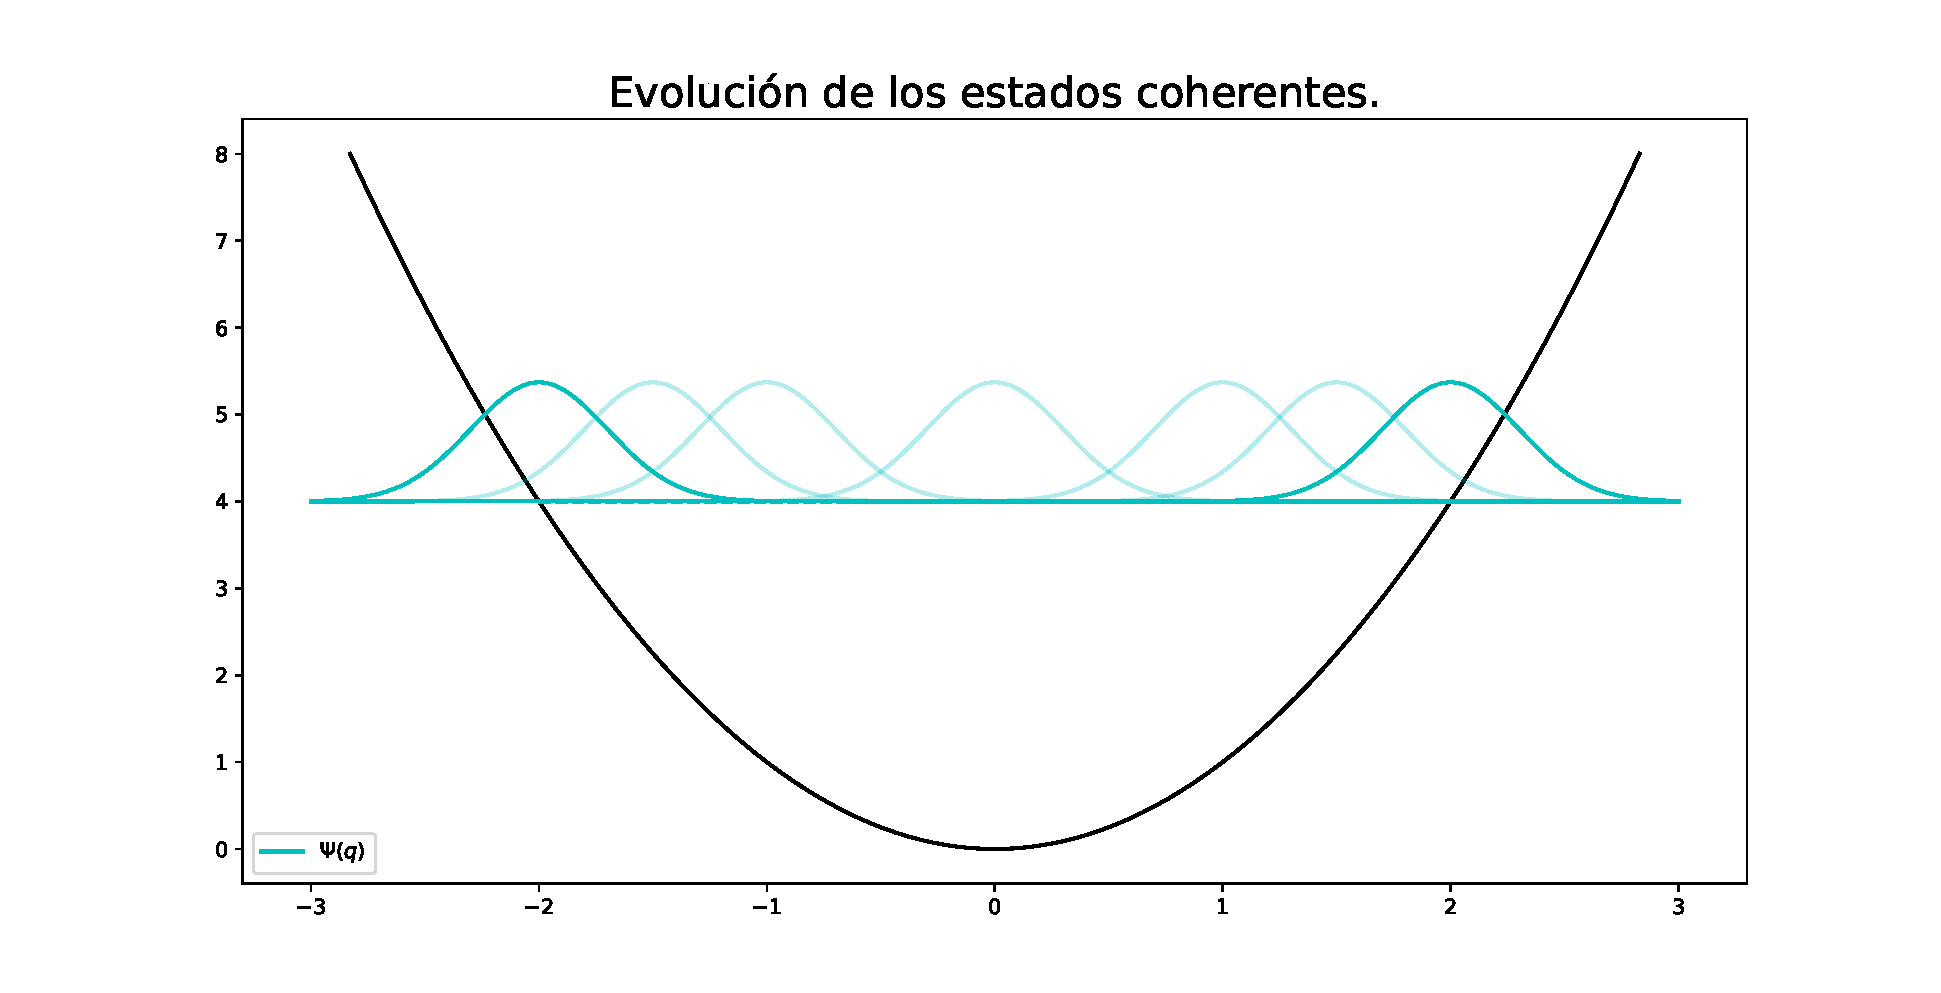
\includegraphics[width = \textwidth]{Capitulo 5/Figuras/EvolEstadosCoherentes.pdf}
        \caption{Los estados coherentes oscilan armónicamente a lo largo del potencial entre los puntos de retorno clásicos. Debido a la forma de estos estados, que sus autovalores con el operador de aniquilación correspondan a una representación compleja de los valores medios de los operadores cuadratura apunta a que físicamente estos estados representan la oscilación bien dirigida de la energía de la radiación.}
        \label{fig:EvolEstadosCoherentes}
    \end{figure}

    Esto se puede también ver un poco más matemáticamente representando estos estados en la base $q$ donde, recordemos, está relacionada con el operador cuadratura $\hat{X}_1$ de la siguiente forma,

    \begin{equation}
        \hat{q} = \sqrt{\frac{\hbar}{2\omega}}(\hat{a} + \hat{a}^{\dagger}) = \sqrt{\frac{2\hbar}{\omega}}\hat{X}_1\;,
    \end{equation}

    \begin{equation}
        \psi_{\alpha}(q) = \braket{q|\alpha} = \left(\frac{\omega}{\pi \hbar} \right)^{1/4}e^{-|\alpha|^2/2}e^{-\xi^{2}/2}\sum_{n=0}^{\infty}\frac{(\alpha /\sqrt{2})^n}{n!}H_n(\xi),
    \end{equation}

    donde $\xi = q\sqrt{\frac{\omega}{\hbar}}$ y $H_n$ son los polinomios de Hermite, mediante la generatriz de los polinomios de Hermite se puede reescribir esta ecuación de forma más compacta así:

    \begin{equation}
        \psi_{\alpha}(q) = \left(\frac{\omega}{\pi\hbar} \right)^{1/4}e^{-|\alpha|^2/2}e^{\xi^2/2}e^{-(\xi-\alpha/\sqrt{2})^2}\;.
    \end{equation}

    Aplicando la evolución temporal tenemos entonces

    \begin{equation}
        \psi_{\alpha}(q,t) = \left(\frac{\omega}{\pi\hbar} \right)^{1/4}e^{-|\alpha|^2/2}e^{\xi^2/2}e^{-(\xi-\alpha e^{-i\omega t}/\sqrt{2})^2}\;.
    \end{equation}
    
    \subsection{Distribución de probabilidad de los estados coherentes}

    Que las fluctuaciones ( o desviación estándar) del número de cuantos $n$ coincida con la magnitud de $\alpha$ nos da pistas de que tal vez la distribución de probabilidad que gobierna estos estados sea una estadística Poissionana \cite{swendsen2020introduction}. De hecho, cuando queremos medir el número de cuantos del campo, la probabilidad de detectar $n$ de estos es

    \begin{equation}\label{eq:PoissonForN}
        P_n = \left|\braket{n|\alpha}\right|^2 = e^{-|\alpha|^2}\frac{|\alpha|^{2n}}{n!} = e^{-\langle n \rangle}\frac{\langle n \rangle^{n}}{n!}.
    \end{equation}

    La ecuación \ref{eq:PoissonForN} es en realidad una densidad de probabilidad de tipo Poisson con valor medio igual a $\langle n \rangle$, podemos ver el comportamiento de esta distribución de probabilidad en la figura \ref{fig:HistogramaEstadosNumero}. 

    \begin{figure}[htbp]
        \centering
        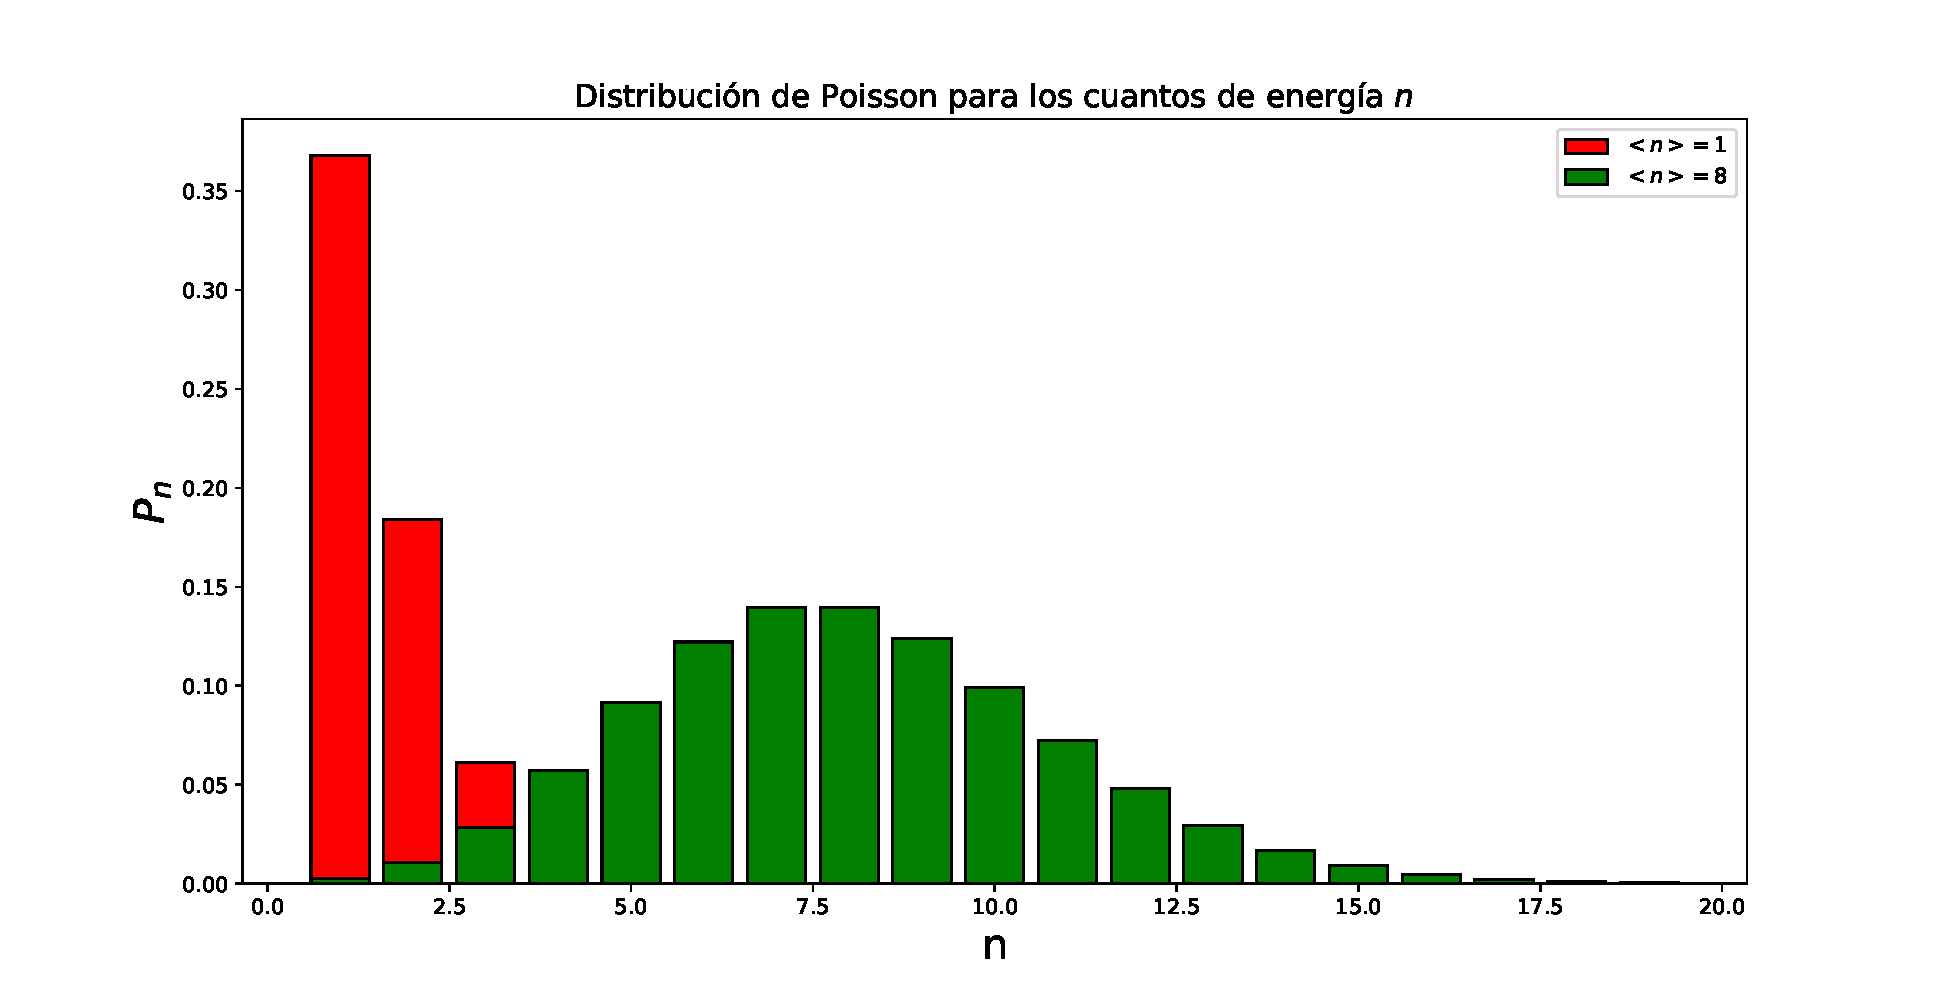
\includegraphics[width = \textwidth]{Capitulo 5/Figuras/HistogramasEstadoNumero.pdf}
        \caption{Densidad de probabilidad para los estados número coherentes.}
        \label{fig:HistogramaEstadosNumero}
    \end{figure}
    
    
    Ahora, veamos también la distribución de fase para los estados coherentes, aquí no entraremos en gran detalle sobre qué es la fase cuántica y cómo operar sobre esta (este tema se discutirá más adelante), gracias a que $\alpha$ es un número complejo este puede ser representado en forma polar $\alpha = |\alpha|e^{i\theta}$ pero como ya vimos este parámetro puede ser representado como $\alpha = \langle \hat{X}_1 \rangle + i \langle \hat{X}_2 \rangle$.
    

    Entonces la correspondiente distribución de fase \cite{gerry2005introductory} es

    \begin{equation}\label{eq:PdePhixd}
        P(\phi) = \frac{1}{2\pi}\left|\braket{\phi|\alpha}\right|^2 = \frac{1}{2\pi}e^{-|\alpha|^2}\left|\sum_{n=0}^{\infty}e^{in(\phi - \theta)} \frac{|\alpha|^{n}}{\sqrt{n!}}\right|^2.
    \end{equation}

    Para valores grandes de cuantos de energía o lo que es lo mismo para valores grandes de $|\alpha|^2$ la distribución de Poisson se aproximará a una Gaussiana:

    \begin{equation}
        e^{-|\alpha|^2} \frac{|\alpha|^{2n}}{n!} \approx \left(2\pi |\alpha|^2\right)^{-1/2} e^{\left[- \frac{(n-|\alpha|^2)^2}{2|\alpha|^2} \right]}
    \end{equation}

    de esta forma la ecuación \ref{eq:PdePhixd} se aproxima al a siguiente forma Gaussiana

    \begin{equation}
        P(\phi) \approx \left(\frac{2|\alpha|^2}{\pi}\right)^{1/2}e^{-2|\alpha|^2(\phi - \theta)^2}\;.
    \end{equation}

    Esta es una densidad de probabilidad Gaussiana cuyo pico se encuentra cuando $\phi = \theta$ y cuyo ancho, igual a $1/(2|\alpha|)$, es inversamente proporcional a $|\alpha|$, es decir, cuanto más grande es el valor medio de cuantos de energía más localizada está la distribución Gaussiana, esto se puede ver en la figura \ref{fig:DistriFaseCoherent}.\\

    \begin{figure}[htbp]
        \centering
        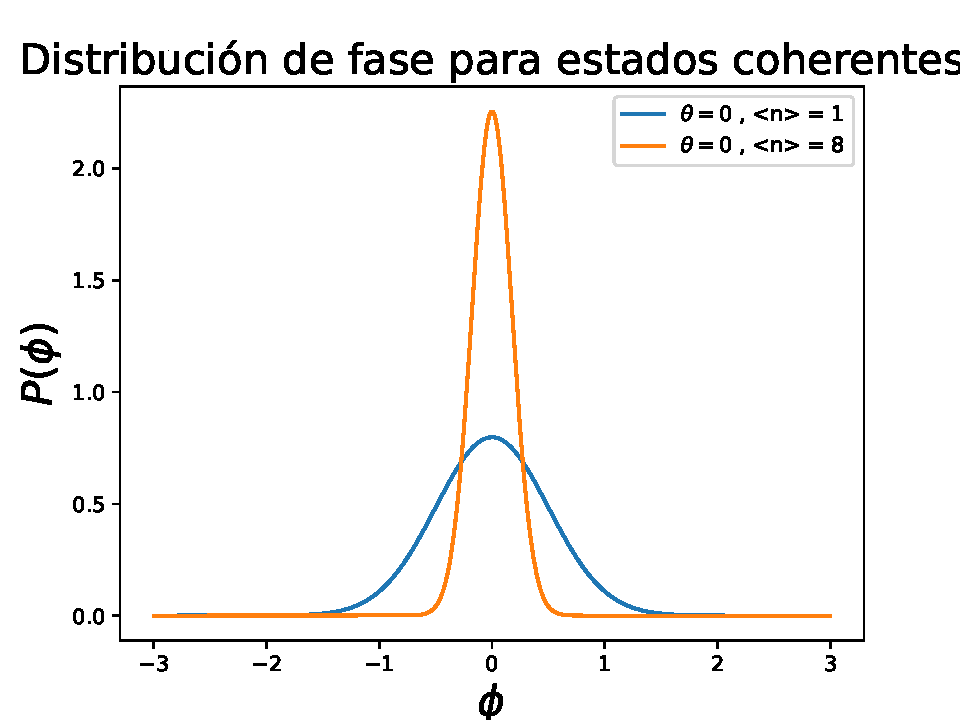
\includegraphics[width = 0.7\textwidth]{Capitulo 5/Figuras/DistribucionDeFaseCoherentes.pdf}
        \caption{Distribución de fase para los estados coherentes, en los cuales se ilustran dos estados centrados en el origen y con dos valores medios del número de cuantos de energía distintos.}
        \label{fig:DistriFaseCoherent}
    \end{figure}

    Podemos concluir que para los estados coherentes $\ket{\alpha}$ son estados cuánticos muy cercanos a estados clásicos porque:

    \begin{enumerate}
        \item El valor esperado del campo eléctrico tiene la forma de la expresión clásica.

        \item Las fluctuaciones en las variables del campo eléctrico son las mismas que para un vacío.

        \item Las fluctuaciones en la incertidumbre fraccional ($\frac{\Delta n}{\langle \hat{n} \rangle} = \frac{1}{\sqrt{\langle \hat{n}\rangle}}$) del número de cuantos de energía disminuyen a medida que aumenta el número promedio de estos.

        \item Los estados se vuelven bien localizados en fase a medida que aumenta el número promedio de fotones.
    \end{enumerate}
